\documentclass[monografia]{ppgccufscar}
%\hyphenation{op-tical net-works semi-conduc-tor}


%\usepackage[latin1]{inputenc}
%\usepackage[brazil]{babel}
%\usepackage[T1]{fontenc}

\usepackage[brazil]{babel}
\usepackage[utf8]{inputenc}
\usepackage[pdftex]{graphicx}
\usepackage{ifpdf}
\usepackage[alf]{abntcite}
\usepackage{subfig}
\usepackage{algorithm2e}
\usepackage{url}
\usepackage{enumerate}
\usepackage{indentfirst}
\setlength{\parindent}{0cm}


\titulo{xxxxxxxxxxxxxxxxxxxxxx}
%\titulo{Proxy RouteFlow Baseado em Java Usando o Controlador Floodlight}
\autor{DAVI GONÇALES PETERLINI \\ FERNANDO CAPPI \\ LUIZ GUSTAVO MAION} 
\orientador[Orientador]{XXXXXXXXXXXXXXXXXX}
%\coorientador[Coorientador]{Dr. Christian Esteve Rothenberg}
%\areaconcentracao{Sistemas Distribuídos e Redes}
\data{2013}


\begin{document} 

\capa
\folhaderosto
\dataaprovacao{00}{Dezembro}{2013}
\begin{folhadeaprovacao}
\examinador{Prof. Dr. XXXXXXXXXXX }{USF - Itatiba}
\examinador{Prof. Dr. XXXXXXXXXXX }{USF - Itatiba}
\end{folhadeaprovacao}

\begin{resumo}

Nos últimos anos o protocolo \textit{OpenFlow} 
vem aumentando a visibilidade das tecnologias 
de redes definidas por software, fazendo com 
que um número cada vez maior de pesquisadores 
e desenvolvedores o adotem como principal
 ferramenta para simulações ou aplicações em
 ambientes reais. O projeto comunitário
 \textit{RouteFlow}, liderado pela Fundação 
\textit{CPqD}, propõe uma plataforma de 
roteamento IP definido por software (do
 termo em inglês, \textit{software-defined networking}) 
baseado no protocolo \textit{OpenFlow}, que permite 
uma separação efetiva do plano de controle do plano 
de encaminhamento dos equipamentos de rede. O 
fato do sistema ter sido criado com o código totalmente
 aberto fez com que o número de usuários aumenta-se 
consideravelmente incentivando a equipe de 
desenvolvedores a atualizá-la constantemente 
para agregar cada vez mais ferramentas e 
tecnologias. O \textit{RouteFlow} faz a 
manipulação do protocolo \textit{OpenFlow} 
utilizando os softwares de controle mais famosos 
da literatura, o \textit{NOX}, criado totalmente 
em \textit{C++} e o \textit{POX}, criado 
totalmente em \textit{Python}. Para aumentar a 
capacidade do \textit{RouteFlow} o trabalho em 
questão descreve a adição de suporte à um novo 
software de controle, o \textit{Floodlight}, sendo 
criado totalmente em \textit{Java}. Sendo assim 
o \textit{RouteFlow} ganhará suporte a mais uma
 tecnologia mantendo-se sempre na vanguarda
 das tecnologias de redes definidas por software.     

\palavraschave{Redes Definidas por Software}
\end{resumo}

\begin{abstract}

In the last years the \textit{OpenFlow} 
protocol has increased the visibility of the software
 defined network technologies, causing a growing 
number of researchers and developers to adopt it as 
the main tool for simulations or applications in real 
environments. The \textit{RouteFlow} community 
project, led by CPqD Foundation, proposes a platform
 defined by IP routing software based on 
the \textit{OpenFlow} protocol, which allows 
effective separation of the control plane of routing
 equipment plan network. The fact that the system
 has been created with fully open source has caused
 the number of users increases considerably encouraging
 the development team to update it constantly adding 
more and more tools and technologies. 
The \textit{RouteFlow} manipulate  the 
\textit{OpenFlow} protocol using the most famous 
controllers of the literature, \textit{NOX}, created 
entirely in \textit{C++} and \textit{POX}, created 
entirely in Python. To increase the capacity of 
the \textit{RouteFlow}, this work describes the 
addiction of the support for a new controller, 
\textit{Floodlight}, being created entirely in 
\textit{Java}. Thus the \textit{RouteFlow} win 
support more technology always staying at the
 forefront of the software defined network technologies.

\keywords{Software Defined Network}
\end{abstract}

\listoffigures
\listoftables

%% defina aqui o seu glossario
\acronym{ISP}{\textit{Internet Service Provider}}
\acronym{IP}{\textit{Internet Protocol}}
\acronym{UDP}{\textit{User Datagram Protocol}}
\acronym{TCP}{\textit{Transmission Control Protocol}}
\acronym{OF}{\textit{OpenFlow}}
\acronym{ARP}{\textit{Address Resolution Protocol}}
\acronym{MPLS}{\textit{Multiprotocol Label Switching}}
\acronym{IPC}{\textit{Inter-Process Communication}}
\acronym{REST}{\textit{Representational State Transfer}}
\acronym{OSPF}{\textit{Open Shortest Path First}}
\acronym{BGP}{\textit{Border Gateway Protocol}}
\acronym{RIP}{\textit{Routing Information Protocol}}
\acronym{JSON}{\textit{JavaScript Object Notation}}
\acronym{API}{\textit{Application Programming Interface}}
\acronym{SNMP}{\textit{Simple Network Management Protocol}}
\listofacronyms

%% sumario
\tableofcontents

\chapter{Introdução}

\section{Objetivo do Trabalho}
O trabalho tem como objetivo principal agregar uma
 nova funcionalidade ao Projeto \textit{RouteFlow}. A 
funcionalidade será o suporte nativo ao controlador 
\textit{Floodlight}. Os controladores são usados 
pelo 
\textit{RouteFlow} como uma interface de comunicação
 entre os softwares de roteamento e os \textit{switches} 
\textit{Openflow}. Cada controlador possui certas
 características juntamente com recursos exclusivos e 
com isso esperá-se que o \textit{RouteFlow} agregue
 as melhores ferramentas disponíveis no controlador 
\textit{Floodlight}.
 A implementação atual do RouteFlow possui suporte
 aos controladores \textit{NOX} e \textit{POX}, sendo 
desenvolvidos respectivamente em C++ e Python. O
 Floodlight foi totalmente desenvolvido em \textit{Java} 
tendo suporte ao estilo de comunicação distribuída
 \textit{REST (Representational State Transfer)}, 
sendo possível utilizado sem a necessidade de programação,
  através de mensagens \textit{REST}.

\section{Contribuições}
Como principal contribuição do trabalho podemos citar
 a integração que haverá entre o \textit{RouteFlow} 
e a comunidade de usuários do controlador \textit{Floodlight}. 
A comunidade poderá realizar simulações 
ou até experimentos em ambientes reais contribuindo ainda
 mais com o avanço do \textit{RouteFlow}. O uso
constante do controlador \textit{Floodlight} pelo
 \textit{RouteFlow} servirá como uma plataforma de testes
para o próprio controlador, contribuindo para a localização de
 possíveis erros ou até mesmo falta de estabilidade.
Outra 
contribuição importante que pode ser citada é a absorção pelo
  \textit{RouteFlow} das melhores 
ferramentas providas pelo \textit{Floodlight}, tornando-o
 cada vez mais completo.  

\chapter{Redes Definidas por Software}

\section{Definição Geral} As Redes Definidas
por Software (Software Defined Networks, ou SDN) constituem
um novo paradigma para o desenvolvimento de pesquisas em
redes de computadores que vem ganhando a atenção de grande
parte da comunidade acadêmica e da industria da área de
redes. Fazendo um balanço geral da situação que encontramos
hoje, podemos dizer que é um pouco complexa: é possível afirmar
que a área de redes fez um sucesso estrondoso, já que hoje a
tecnologia de redes de computadores permeia todos os níveis
da sociedade. Grande parte das atividades da sociedade de
alguma forma passa por uma ou mais redes de computadores.

Mas tamanho sucesso trouxe consigo um problema para a comunidade
de pesquisa. Como grande parte da sociedade depende hoje da
internet em suas atividades diárias e as tecnologias de rede
se tornaram de fácil acesso, a estabilidade se tornou uma
característica fundamental das redes de computadores. Isso
significa que pesquisas com novas tecnologias e protocolos
já não são mais possíveis em redes de larga escala, como a
Internet, devido ao risco de interrupção ou instabilidade
dos serviços essenciais. Outro problema encontrado pelos
pesquisadores é o fato de que a larga utilização de
tecnologias já desenvolvidas inviabiliza a inserção de
qualquer tecnologia que exija a inserção de novos
equipamentos de hardware.

Mesmo pesquisadores trabalhando em redes experimentais sofrem
para justificar a adoção em larga escala das tecnologias
desenvolvidas nesses ambientes. O potencial de instabilidade
ou ruptura de tais avanços se torna um forte argumento
contra sua adoção.

Esses problemas citados acima só ocorrem pelo fato de que redes
de computadores em geral e a rede mundial (a Internet)
atingiram um nível de amadurecimento que as tornaram pouco 
flexíveis.
Para tentar melhorar essa situação, a comunidade de pesquisa
em redes de computadores tem investido em iniciativas que
levam ao desenvolvimento de redes com maiores 
recursos de programação, de forma que as novas tecnologias
possam ser inseridas na rede de forma gradual. Exemplos de
iniciativas desse tipo são as propostas de redes ativas
\textit{(active networks)} [Tennenhouse e Wetherall 2007],
de \textit{testbeds} como o PlanetLab [Peterson e Roscoe 2006]
e, mais recentemente, do GENI [Turner 2006, Elliott e Falk
2009]. Redes ativas, apesar de terem grande potencial,
tiveram pouca aceitação pela necessidade de alteração dos
elementos de rede para permitir que se tornassem programáveis. As iniciativas 
mais recentes, como o PlanetLab e o GENI, apostam na adoção
de recursos de virtualização para facilitar a transição para
novas tecnologias. Apesar de serem consideradas de
grande potencial ao longo prazo, tais iniciativas ainda
enfrentam desafios em questões como garantir o desempenho
exigido pelas aplicações largamente utilizadas hoje
utilizando-se tais elementos de rede virtualizados.

Uma outra forma de abordar o problema, a fim de oferecer
um caminho de menor impacto e que possa ser implementado 
em prazos mais curtos e com bom desempenho, consiste
em estender o hardware de encaminhamento de pacotes
de forma mais restrita. Considerando-se que a operação 
que precisa de alto desempenho nos elementos de comutação
atual é o encaminhamento de pacotes, algumas iniciativas
propõem manter essa operação pouco alterada, para manter 
a viabilidade de desenvolvimento de hardware de alto
desempenho, mas com uma possibilidade de maior controle 
por parte dos administradores de rede. Essa proposta se inspira 
em uma tecnologia já largamente adotada, o chaveamento
(encaminhamento) baseado em rótulos programáveis, 
popularizado pelo MPLS \textit{(Multi-Protocol Label
 Switching)} [Davie e Farrel 2008, Kempf et al. 2001].

Com o MPLS, o controle fino sobre o tráfego de rede se torna 
possível ao se atribuir a cada pacote um rótulo \textit{(label)}
que determina como o mesmo será tratado pelos elementos
de rede. Explorando esse recurso, administradores de rede podem
exercer controle diferenciado sobre cada tipo de tráfego de rede,
assumindo que os mesmos possam ser identificados para
receberem os rótulos apropriados. Com base nessa observação,
uma ideia trabalhada por diversos pesquisadores é a manutenção 
de um hardware de encaminhamento de alto desempenho, com
a possibilidade de permitir que os administradores de redes (ou 
os desenvolvedores de aplicações para a rede) determinem como 
os fluxos irão ser rotulados e encaminhados.

A iniciativa mais bem sucedida nesse sentido foi, sem dúvida,
definição da interface e do protocolo OpenFlow [McKeown et al.
2008]. Com o OpenFlow, os elementos de encaminhamento 
oferecem uma interface de programação simples que lhes
permite estender o acesso e controle da tabela de consulta 
utilizada pelo hardware para determinar o próximo passo de 
cada pacote recebido. Dessa forma, o encaminhamento continua 
sendo eficiente, pois a consulta à tabela de encaminhamento 
continua sendo tarefa do hardware, mas a decisão sobre 
como cada pacote deve ser processado pode ser transferida
para um nível superior, onde diferentes funcionalidades 
podem ser implementadas. Essa estrutura permite que a rede
seja controlada de forma extensível através de aplicações,
expressas em software. A esse novo paradigma, deu-se o 
nome de Redes Definidas por Software, ou \textit{Software
Defined Networks} (SDN).

Do ponto de vista histórico, as Redes Definidas por 
Software têm sua origem na definição
da arquitetura de redes \textit{Ethane}, que definia uma forma
de se implementar políticas de controle de acesso de forma 
distribuída, a partir de um mecanismo de supervisão centralizado
[Casado et al. 2009]. Naquela arquitetura, cada elemento de 
rede deveria consultar o elemento supervisor ao identificar um
novo fluxo. O supervisor consultaria um grupo de políticas 
globais para decidir, com base nas características de cada
fluxo, como o elemento de encaminhamento deveria 
tratá-lo. Essa decisão seria comunicada ao comutador na 
forma de programação de uma entrada em sua tabela de
encaminhamento com uma regra adequada para o novo fluxo (
que poderia, inclusive, ser seu descarte). Esse modelo foi
posteriormente formalizado por alguns autores na forma da 
arquitetura \textit{OpenFlow}.

\section{Introdução ao Protocolo \textit{OpenFlow}}

O \textit{OpenFlow} foi proposto pela Universidade de
Stanford para atender à demanda de validação de novas
propostas de arquiteturas e protocolos de rede (incluindo as
abordagens \textit{clean slate}) sobre equipamentos
comerciais. É definido como uma padrão aberto para Redes
Definidas por Software que tem como principal objetivo que 
se utilize equipamentos comerciais para pesquisa e 
experimentação de novos protocolos de rede, em paralelo
com a operação normal das redes. Isso é conseguido com a 
definição de uma interface de programação que permite 
ao desenvolvedor controlar diretamente os elementos de 
encaminhamento de pacotes presentes no dispositivo. Com o 
\textit{OpenFlow}, pesquisadores podem utilizar equipamentos de 
rede comerciais, que normalmente possuem maior poder 
de processamento que os comutadores utilizados em 
laboratórios de pesquisa, para realizar experimentos em redes
"de produção". Isso facilita muito a transferência dos resultados
de pesquisa para a industria. 

\section{Descrição Geral do Protocolo \textit{OpenFlow}}

Uma característica básica da arquitetura do padrão \textit{OpenFlow} 
é a separação clara entre os planos de dados e controle em
elementos de chaveamento. O plano de dados cuida do 
encaminhamento de pacotes com base em regras simples (chamadas de ações 
na terminologia \textit{OpenFlow}) associadas
a cada entrada da tabela de encaminhamento do comutador 
de pacotes (podendo ser um \textit{switch}, um roteador 
ou até mesmo um ponto de acesso sem fio).
Essas regras, definidas pelo padrão, incluem (\textit{i}) 
encaminhar o pacote para uma porta especifica do dispositivo,
(\textit{ii}) alterar parte de seus cabeçalhos, (\textit{iii}) 
descartá-los, ou (\textit{iv}) encaminhá-lo para inspeção 
por um controlador da rede. Em dispositivos dedicados, o plano
de dados pode ser implementado em hardware utilizando os
elementos comuns aos roteadores e \textit{switches} atuais.
Já o módulo de controle (ou controlador) pode ser um 
módulo de software implementado de forma independente em
algum ponto da rede.

A principal abstração utilizada na especificação
\textit{OpenFlow} é o conceito
de fluxo. Um fluxo é constituído pela combinação de campos
do cabeçalho do pacote a ser processado pelo dispositivo,
conforme Figura \ref{fig:cabecalhoOpenflow}. As tuplas podem
ser formadas por campos das camadas de enlace, de rede ou de
transporte, segundo o modelo \textit{TCP/IP}. Deve-se
enfatizar que a abstração da tabela de fluxos ainda está sujeita a
refinamentos, com o objetivo de oferecer uma melhor
exposição dos recursos do hardware e, nesse caso, permitir a
concatenação de várias tabelas já disponíveis, como, por
exemplo, tabelas \textit{IP/Ethernet/MPLS}. Nesse sentido, a
contribuição mais importante do paradigma do
\textit{OpenFlow} é a generalização do plano
de dados – qualquer modelo de encaminhamento de dados
baseado na tomada de decisão fundamentada em algum valor, ou
combinação de valores, dos campos de cabeçalho dos pacotes
pode ser suportado.

\begin{figure}[hb] \centering
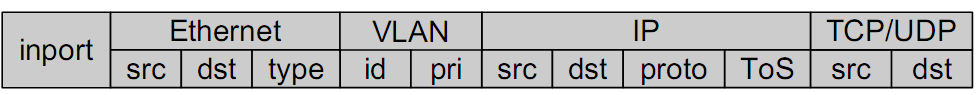
\includegraphics[width=160mm]{cabecalhoOpenflow.png}
\caption{Cabeçalho \textit{OpenFlow} para a especificação dos fluxos}
\label{fig:cabecalhoOpenflow}
\end{figure}

Um grande trunfo da arquitetura \textit{OpenFlow} é a flexibilidade 
que ela oferece para se programar de forma independente do
tratamento de cada fluxo observado, do ponto de vista de como
o mesmo deve (ou não) ser encaminhado pela rede. Basicamente,
o padrão \textit{OpenFlow} determina como um fluxo pode ser definido,
as ações que podem ser realizadas para cada pacote pertencente
a um fluxo e o protocolo de comunicação entre o comutador de 
pacotes e o controlador, utilizado para realizar alterações dessas 
definições e ações. A união de uma definição de fluxo e um
conjunto de ações forma uma entrada da tabela de fluxos 
\textit{OpenFlow} [McKeown et al. 2008].

Em um \textit{switch} \textit{OpenFlow}, cada entrada na tabela de 
fluxos pode ser implementada como um padrão de bits 
representado em uma memória TCAM (Ternary Content-
Addressable Memory). Nesse tipo de memória, bits podem
ser representados como zero, um ou "não importa" 
(\textit{don't care}), indicando que ambos os valores são
aceitáveis naquela posição. Como o padrão é programado
a partir do plano de controle, fluxos podem ser definidos da 
forma escolhida pelo controlador. A Figura \ref{fig:fluxoopenflow}
apresenta uma visão geral de uma entrada da tabela \textit{OpenFlow}.
Cada pacote que chega a um comutador \textit{OpenFlow} é comparado
com cada entrada dessa tabela; caso um casamento seja encontrado,
considera-se que o pacote pertence àquele fluxo e aplica-se
as ações relacionadas à esse fluxo. Caso um casamento não
seja encontrado, o pacote é encaminhado para o controlador 
para ser processado -- o que pode resultar na criação de uma
nova entrada para aquele fluxo. Além das ações, a arquitetura
prevê a manutenção de três contadores por fluxo: pacotes,
 \textit{bytes} trafegados e duração do fluxo. Esses contadores são 
implementados para cada entrada da tabela de fluxos e 
podem ser acessados pelo controlador através do protocolo
\textit{OpenFlow}.

\begin{figure}[hb] \centering
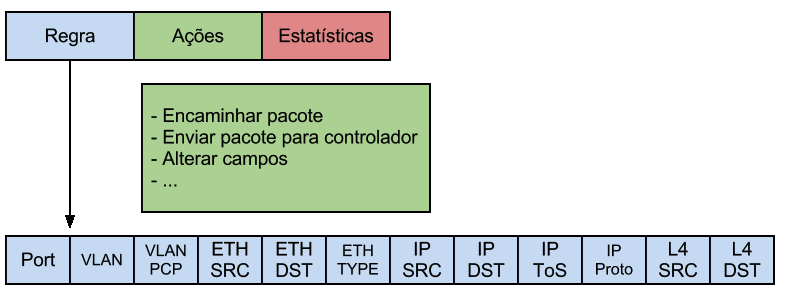
\includegraphics[width=160mm]{fluxoOpenflow.png} 
\caption{Exemplo de uma entrada na tabela de fluxos \textit{OpenFlow}.} 
\label{fig:fluxoopenflow} 
\end{figure}

Esse pequeno conjunto de regras cria diversas possibilidades,
pois muitas das funcionalidades que são implementadas 
separadamente podem ser agrupadas em um único controlador
\textit{OpenFlow}, utilizando um pequeno conjunto de regras. Alguns 
exemplos das possibilidades são apresentadas na Figura \ref{fig:exemploSwitchOpenFlow}.
As entradas representam o uso do \textit{switch} \textit{OpenFlow}
para realizar encaminhamento de pacotes na camada de enlace,
implementar um firewall e realizar encaminhamento de pacotes 
na camada de enlace utilizando redes virtuais (VLANs), respectivamente.

\begin{figure}[h] \centering
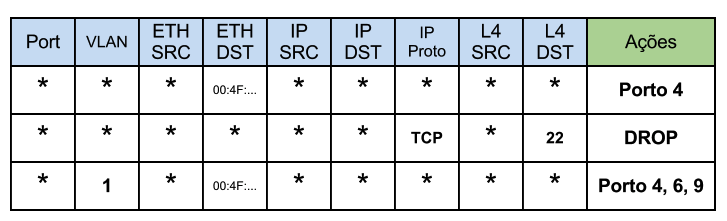
\includegraphics[width=160mm]{exemploSwitchOpenFlow.png} 
\caption{Exemplos de uso de um \textit{switch OpenFlow}.} 
\label{fig:exemploSwitchOpenFlow} 
\end{figure}

Apesar de possuir um conjunto pequeno de ações simples, 
alguns descrevem o \textit{OpenFlow} como uma analogia ao conjunto 
de instruções de um microprocessador x86 que, apesar de 
pequeno e simples, provê uma vasta gama de possibilidades 
para o desenvolvimento de aplicações. O \textit{OpenFlow} cria 
possibilidades semelhantes para o desenvolvimento de 
aplicações no contexto de redes de computadores. 

A versão atual do \textit{OpenFlow} ainda possui algumas limitações
em termos do uso padrão em circuitos ópticos e uma definição 
de fluxos que englobe protocolos que não fazem parte do 
modelo TCP/IP. No entanto, está sendo formulada uma nova
versão cujo objetivo é eliminar algumas dessas limitações.

A Figura \ref{fig:openflow} define de forma introdutória uma 
rede de computadores com o protocolo \textit{OpenFlow} habilitado. Os 
elementos comutadores podem ser de qualquer tipo, como 
comutadores convencionais, roteadores ou até mesmo pontos
de acesso sem fio. Podemos ver o elemento externo, chamado
de controlador, tomando contas das regras e ações instaladas
no hardware de rede. O controlador pode ser executado em 
qualquer equipamento com suporte à redes, como um 
servidor comum.

\begin{figure}[h] \centering
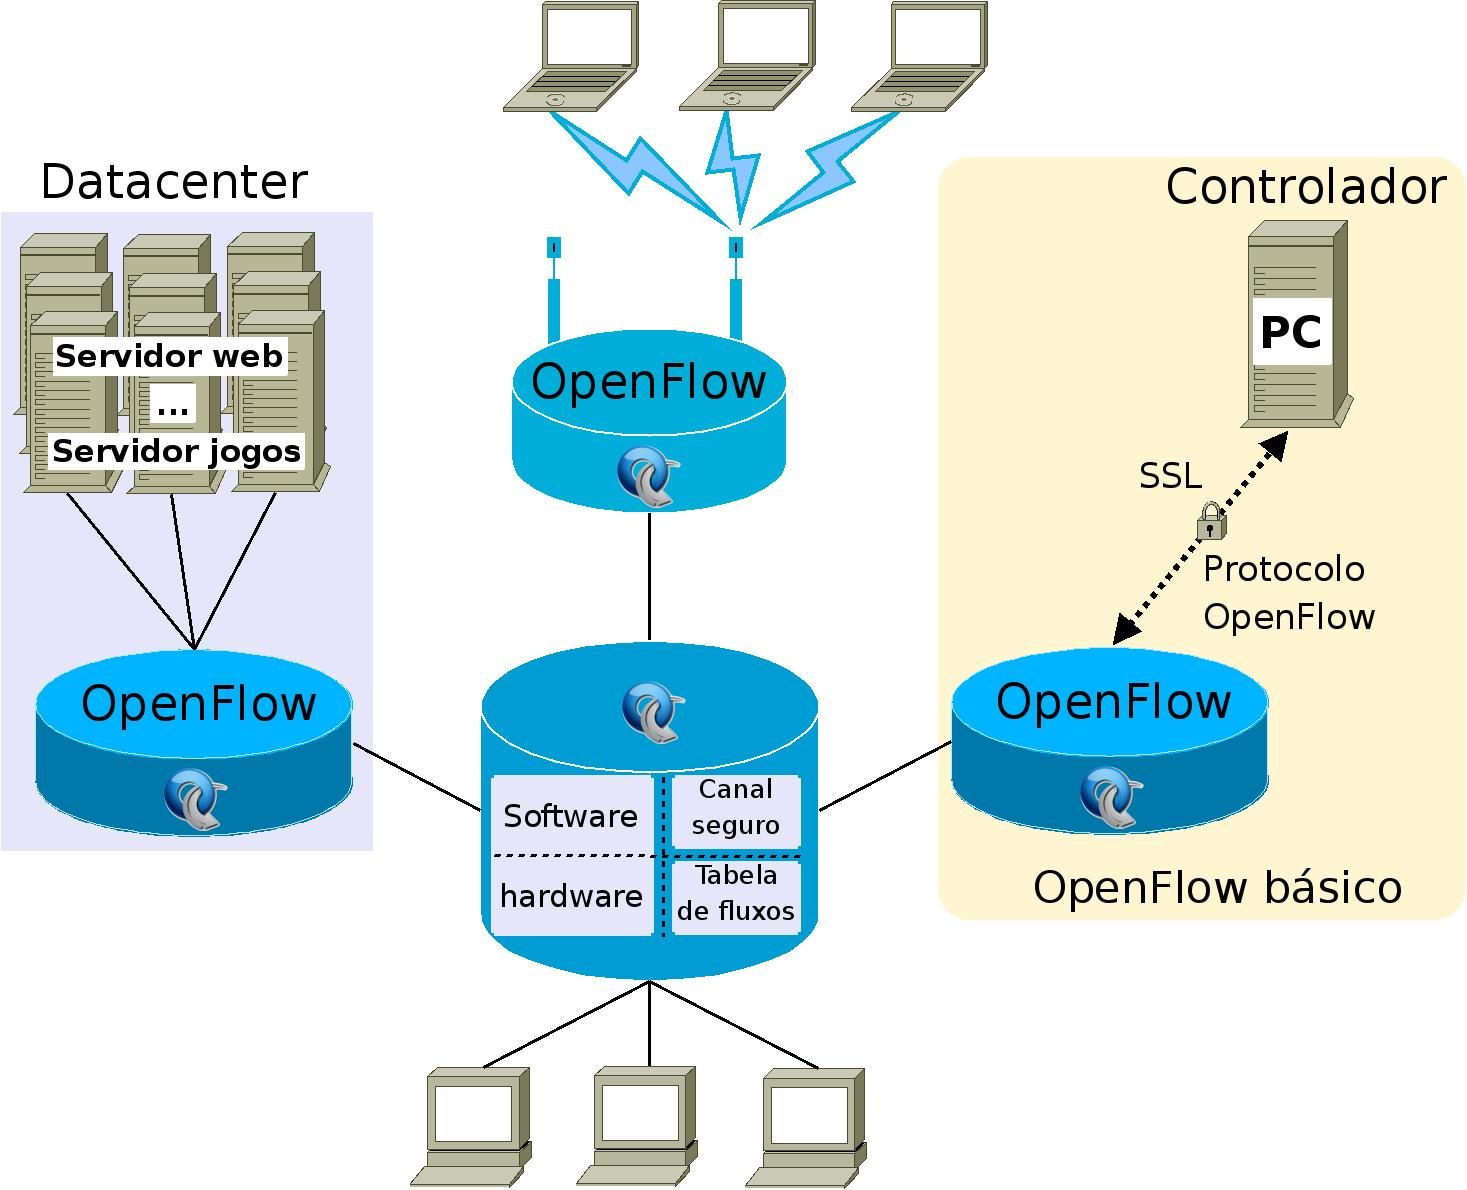
\includegraphics[width=130mm]{openflow.png} 
\caption{Rede com o protocolo \textit{OpenFlow} habilitado.} 
\label{fig:openflow} 
\end{figure}
\chapter{Arquitetura Básica do RouteFlow}

\section{Introdução ao Projeto Comunitário RouteFlow}

O projeto comunitário RouteFlow é uma proposta de oferta de serviços de
roteamento IP remoto de forma centralizada, e que visa um
desacoplamento efetivo entre o plano de encaminhamento e o
plano de controle (ROUTEFLOW, 2011). O objetivo é tornar as
redes IP mais flexíveis pela facilidade de adição,
remoção e especialização de protocolos e algoritmos.


O RouteFlow prove um serviço virtualizado de roteamento IP
em equipamentos com suporte ao protocolo \textit{OpenFlow}
seguindo o paradigma das redes definidas por software.
Basicamente, o RouteFlow interliga uma infraestrutura 
\textit{OpenFlow} com um ambiente virtual de roteamento 
IP baseado em ferramentas nativas do Linux (Quagga) para
um roteamento eficiente na estrutura física. Baseado em um
sistema de controle RouteFlow, os \textit{switches} 
são instruídos via controladores \textit{OpenFlow} que 
trabalham como proxies no intuito de traduzir as mensagens
e eventos entre o ambiente físico e virtual. 

O projeto conta com um número crescente de usuários no 
mundo (cerca de 1000 downloads e mais de 10000 visitantes
desde que o projeto começou em Abril de 2010). As principais
formas de contribuição para o projeto é através do sistema
de repositórios GitHub. Para citar alguns exemplos de contribuição
por parte da comunidade, é possível citar a contribuição
do Google nos plugins SNMP e o trabalho atual no suporte
ao MPLS e nas APIs de roteamento Quagga. A universidade
americana de Indiana contribuiu com uma interface gráfica
e com a execução de um piloto em seu \textit{testbed}.
% É possível adicionar mais exemplos de contribuições externas


O RouteFlow é composto basicamente por três módulos principais:
o cliente RouteFlow (RFClient), o servidor RouteFlow (RFServer) e
o proxy RouteFlow (RFProxy). Todos os módulos serão
explicados com mais detalhes nas seções seguintes. A Figura \ref{fig:visaoGeralRouteFlow} mostra
de forma simplificada um cenário RouteFlow típico: engines de 
roteamento em um ambiente virtual geram uma base de 
informação de encaminhamento baseado nos protocolos 
de roteamento (OSPF, BGP) e processos ARP. Durante a 
execução do ambiente virtual, as tabelas de roteamento e 
tabelas ARP são coletadas pelos módulos clientes (RFClient) executando
nas máquinas virtuais e traduzidas em tuplas OpenFlow que
são enviadas para o servidor (RFServer), que faz a adaptação das 
informações para o ambiente físico e finalmente instrui o 
módulo proxy (RFProxy), uma aplicação controladora, para configurar
os \textit{switches OpenFlow} no ambiente físico.


\begin{figure}[h]
\centering
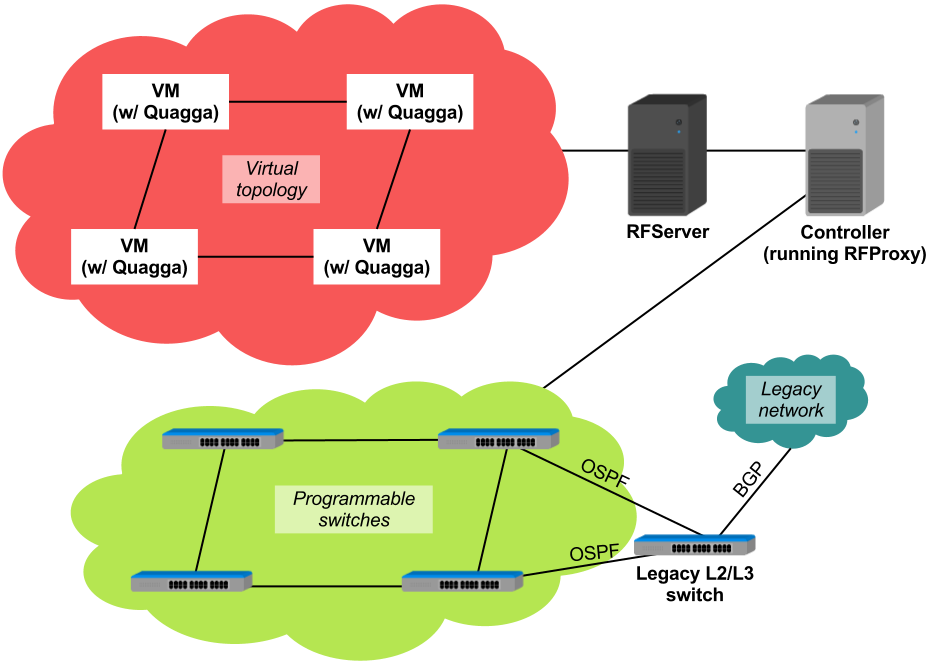
\includegraphics[width=160mm]{visaoGeralRouteFlow.png}
\caption{Visão geral do RouteFlow.}
\label{fig:visaoGeralRouteFlow} 
\end{figure}


Pacotes de encaminhamento dos protocolos de roteamento 
e controle de tráfico (ARP, BGP, RIP e OSPF) são direcionados
pelo proxy RouteFlow para as interfaces virtuais correspondentes do
ambiente virtual. Entre o ambiente virtual e o ambiente existe
um \textit{switch} virtual que também é controlado pelo proxy RouteFlow,
permitindo um caminho direto entre os ambientes, reduzindo 
o tempo das trocas de mensagens e sem a necessidade de passar
através do servidor RouteFlow e do cliente RouteFlow.

Abaixo temos os principais avanços da arquitetura do projeto
RouteFlow

\begin{itemize}
\item \textbf{Plataforma totalmente modular, extensível, 
configurável e flexível.} A arquitetura atual do RouteFlow 
foi feita pensando em sua própria evolução. Através do 
conceito de camadas, o RouteFlow conseguiu facilitar o entendimento
geral do código, facilitando o seu entendimento total por parte de 
seus usuários. A construção baseada em módulos independentes
torna o código mais claro, facilitando a portabilidade para outras 
linguagens ou o suporte à novas tecnologias. O exemplo mais 
claro sobre a independência dos módulos é o próprio módulo levado em consideração
na construção do trabalho de conclusão de curso em questão, o
proxy RouteFlow. 

O proxy RouteFlow faz a troca de mensagens com os outros módulos 
através de um sistema de banco de dados, sendo facilmente
portado para outras linguagens de programação e tecnologias.

Outro beneficio da construção baseada em módulos é a possibilidade
de execução do RouteFlow em múltiplos sistemas computacionais, 
fazendo-o executar como uma arquitetura distribuída. Tal 
característica será melhor explicada nos itens abaixo.
\item \textbf{Suporte à replicação do estado da rede e grande
disponibilidade dos recursos.} Para melhorar a disponibilidade
do sistema, o RouteFlow foi construído de forma descentralizada, 
separando os dados relacionados ao estado das redes dos módulos de processamento.
Todos os dados relacionados ao estado das redes é armazenado
em um banco de dados centralizado, possibilitando que qualquer aplicação 
registrada tenha acesso. Dessa maneira é possível obter uma 
replicação dos processos, obtendo as vantagens e benefícios
de um sistema descentralizado. 

A versão atual do projeto ainda
não faz duplicação dos processos mas a ideia já é levada em
consideração para futuras implementações. 
\item \textbf{Armazenamento do histórico da rede e de estatísticas.}
Como citado no item anterior, a ideia de descentralização do RouteFlow
fez que os dados fossem armazenados em um banco de 
dados centralizado. Esse características traz consigo
uma série de vantagens, além de todas citadas anteriormente, ainda pode ser 
mencionado a possibilidade
de se manter um histórico das ações e decisões tomadas pelo
sistema. O RouteFlow, através do banco de dados centralizado, mantem 
um histórico de todo o sistema, bem como as estatísticas relacionadas 
à criação de regras e ao uso da rede. Tais características permitem
 aos pesquisadores
ou até mesmo aos administradores de redes ter um controle 
e um entendimento mais elaborado, podendo reproduzir o ambiente
em certos períodos de tempo. É possível reproduzir o sistema
em ambientes em que o mesmo apresentou certa irregularidade ou
falha. 
As estatística ainda dão ao administrador um entendimento maior 
de como a rede é usada, possibilitando ao mesmo a tomada de
alguma decisão para a busca de melhorias.
\item \textbf{Possibilidade de ambientes com múltiplos controladores
\textit{OpenFlow}.} A arquitetura atual do RouteFlow foi
desenvolvida para ter suporte em cenários com múltiplos controladores
\textit{OpenFlow}. Tal característica permite aos pesquisadores
ou administradores particionar a rede e controlar cada região
com um controlador independente. Outro fator interessante é
que as camadas superiores do RouteFlow abstraem as diferenças
entre as versões 1.0/1.1/1.2/1.2 do OpenFlow, tornando fácil o
suporte à controladores heterogêneos. 
Para que tal característica fosse suportada, o código do RouteFlow
passou por um processo de padronização, melhorando ainda 
mais a legibilidade do projeto.
\end{itemize}

% Melhorar o titulo
\section{Banco de Dados Centralizado com Suporte à Mecanismo
de Troca de Mensagens Entre Processos}

Nesse capitulo será explicado com detalhes a arquitetura de 
banco de dados centralizado e seu suporte aos mecanismos
de comunicação entre processos usados pelo projeto RouteFlow.
Também serão abordados as principais vantagens e desvantagens
da arquitetura.

Várias abordagens foram proposta pelo RouteFlow para um
esquema unificado de comunicação entre processos (IPC). 
Inúmeras delas foram testadas e avaliadas até se conseguir 
traçar as principais vantagens e desvantagens de cada uma delas.
Soluções baseadas em filas de mensagens, como o RabbitMQ
ou o ZeroMQ foram descartadas por causa da grande complexidade
de implementação e manutenção. Soluções baseadas em serialização
de mensagens, como ProtoBuffers e Thrift, se apresentaram como
boas soluções mas requiriam uma lógica adicional para o armazenamento
pendente e para mensagens já consumidas. Durante o estudo
de banco de dados Não SQL para armazenamento persistente,
surgiu as primeiras ideias do uso de um banco de dados como
ponto central de um mecanismo de troca de mensagens entre 
processos (IPC) e consequentemente manter o histórico das 
ações tomadas pelo RouteFlow para permitir a replicação de certas
situações.

Depois de levar em consideração as mais populares opções de 
banco de dados Não SQL (MongoDB, Redis e CouchDB), foi 
decidido sobre a implementação de um banco de dados centralizado
e dos mecanismos de troca de mensagens entre processos (IPC) 
utilizando-se o MongoDB. Os principais fatores para a escolha foram
a facilidade de programação, suporte nativo a inúmeras linguagens de 
programação, suporte nativo à tecnologia JSON e a existência de 
mecanismos para replicação e distribuição. A ideia por trás do
mecanismo de troca de mensagens (IPC) é completamente
independente da escolha do banco de dados e por isso não 
foi levada em consideração.

No núcleo do RouteFlow estão os mapeamentos entre o ambiente
físico controlado e o ambiente virtual executando as tarefas de
roteamento. A confiabilidade desses estados de rede é imprescindível 
para o servidor RouteFlow e se torna difícil de manter sem a ajuda de 
algum módulo externo. Um banco de dados externo se encarrega
desse objetivo, tendo sua configuração mais flexível. Estatísticas
coletadas pelo proxy RouteFlow também podem ser armazenadas em 
um banco de dados centralizado, baseado em serviços adicionais
é até possível implementar ferramentas para análise dos dados 
ou até mesmo visualização.

A escolha de delegar o controle dos estados da rede para um
banco de dados permite uma melhor tolerância a falhas, replicando
a base de dados ou até mesmo separando o servidor RouteFlow em várias
instâncias. A possibilidade de distribuição do servidor RouteFlow permite
ao sistema um melhor desempenho, sendo possível distribuí-lo
em vários pontos de uma rede e assim reduzindo a latência de
comunicação. Já é levado em consideração o uso de um banco de
dados distribuído para as próximas atualizações do RouteFlow.

A implementação atual do RouteFlow leva em consideração
as melhores técnicas e práticas usadas em aplicações executando
nas nuvens, isso inclui recursos de escalabilidade, banco de 
dados tolerante à falhas que serve como mecanismo de troca
de mensagens entre processos (IPC), controle centralizado
do estado da rede, armazenamento das informações usadas 
para desenvolvimento de aplicações de roteamento (histograma 
de tráfico, monitoramento de fluxos e ações administrativas).
Assim podemos dizer que o banco de dados nos provê uma 
base com informações da rede (\textit{Network Information
Base, NIB}) [Koponen et al. 2010] e uma base de conhecimento
 (\textit{Knowledge Information Base, KIB}) [Saucez et al. 2011].

\section{Esquema de Configuração Flexível}

Nas primeiras versões do RouteFlow, a associação entre máquinas
virtuais (executando o cliente RouteFlow) e os \textit{switches OpenFlow}
era feita de forma automática e gerenciada pelo servidor RouteFlow baseado
no critério de ordem de registração: o cliente de numero um
era associado ao primeiro \textit{switch} à ingressar na rede, o de número
dois ao segundo e assim diante. Essa característica não requeria 
que o administrador controla-se o registro dos \textit{switches} na rede mas
era necessário tomar conta da ordem de ingresso dos \textit{switches}.

Essa abordagem funcionou bem em ambientes controlados e 
experimentais mas apresentou problemas em ambientes onde
os switches não eram controlados diretamente pelo administrador.
Para resolver este problema e ser base para o suporte ao uso de
múltiplos controladores, a implementação atual do RouteFlow
faz uso de um mapeamento 1:1 definido de forma manual pelo 
administrador da rede.
É necessário o conhecimento prévio da rede pelo administrador
para que o mapeamento seja feito de forma correta. Esse mapeamento
é carregado e armazenado no banco de dados centralizado.
A Tabela \ref{tab:tipos_associacao} demonstra os possíveis estados que o mapeamento
pode assumir. A Figura \ref{fig:rfserverAssociacao} ilustra como o servidor RouteFlow trata os eventos
da rede.


\begin{table}[h]
\centering
\begin{tabular}{|l|c|c|}
\hline
Formato & Tipo\\
\hline
\hline
$vm_-id,vm_-port,-,-,-,-,-$ & Porta do Cliente Inativa\\
\hline
$-,-,-,-,-,dp_-id,dp_-port,ct_-id$ & Porta do Switch Inativa\\
\hline
$vm_-id,vm_-port,dp_-id,dp_-port,-,-,ct_-id$ & Associação entre Cliente e Switch\\
\hline
$vm_-id,vm_-port,dp_-id,dp_-port,vs_-id,vs_-port,ct_-id$ & Associação entre Cliente e Switch Ativa\\
\hline
\end{tabular}
\caption{Tipos possíveis de associação}
\label{tab:tipos_associacao}
\end{table}


Sempre que um \textit{switch} OpenFlow ingressa na rede, o proxy RouteFlow
informa ao servidor RouteFlow sobre cada uma das
portas físicas. Cada uma dessas portas é registrada pelo servidor
em um dos dois tipos mostrados na Tabela \ref{tab:tipos_associacao}:
como (i) \textit{Porta de Switch Inativa} ou (ii) \textit{Associação
entre Cliente e Switch}. Essa associação ocorre quanto 
não há nenhuma configuração para a porta do \textit{switch} que
foi registrada ou a porta cliente configurada para ser associada
com essa porta do \textit{switch} ainda não foi registrada. A última 
opção acontece quando a porta do cliente a ser associada com a
porta do \textit{switch} (baseada na configuração prévia do ambiente)
está pronta e registrada como inativa.

Quando um cliente RouteFlow inicia, o mesmo informa ao servidor RouteFlow 
informações sobre suas interfaces (portas). Essas portas são 
registradas pelo servidor RouteFlow em um dos estados mostrados na
Tabela \ref{tab:tipos_associacao}: como uma porta de cliente
inativa ou como uma associação entre cliente e \textit{switch}. A 
associação é análoga a associação descrita às portas dos
\textit{switches}.

Depois da associação, o servidor RouteFlow solicita ao cliente RouteFlow para
disparar a mensagem que irá confirmar que o \textit{switch} virtual está
conectado e apto a se comunicar com o proxy RouteFlow. Quando isso
acontece, o proxy RouteFlow é alertado sobre a conexão entre o 
cliente RouteFlow e seu \textit{switch} virtual, e envia uma informação ao 
servidor RouteFlow. O servidor RouteFlow decide o que fazer com a informação.
Tipicamente, o proxy RouteFlow é intruido a redirecionar todo o tráfego
das máquinas virtuais para os \textit{switches} físicos associados e 
vice-versa. Quando um \textit{switch} abandona a rede, todas as 
associações envolvendo as portas do mesmo são removidas,
deixando inativas as portas do cliente envolvidas na associação.
Em caso de conexão de um \textit{switch}, o servidor RouteFlow checa se o 
mesmo é um novo ingressante ou se é um retornante, podendo
apenas restaurar as associações configuradas previamente 
pelo administrador.


\begin{figure}[h]
\centering
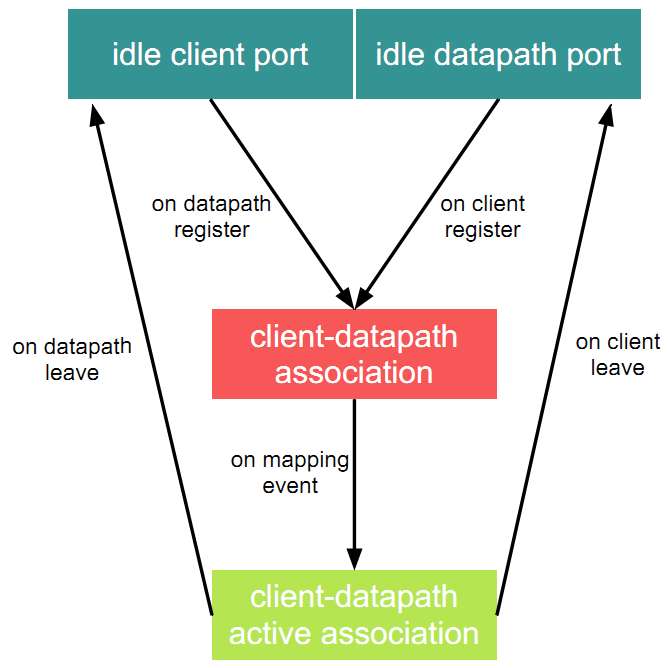
\includegraphics[width=120mm]{rfserverAssociacao.png}
\caption{Tratamento de associações do servidor RouteFlow.}
\label{fig:rfserverAssociacao} 
\end{figure}


Uma entrada no arquivo de configuração contem um conjunto 
dos campos identificados na Tabela \ref{tab:tipos_associacao}:
\textit{$vm_-id, vm_-port, dp_-id, dp_-port, ct_-id$}. Esses campos
são suficientes para a associação, os campos remanescentes
são relacionados à conexão com o \textit{switch} virtual ($vs_-*$) e serão
definidos em tempo de execução. O campo \textit{$ct_-id$} identifica
identifica com qual controlador o \textit{switch} está conectado. Esse
mecanismo permite ao RouteFlow trabalhar com múltiplos
controladores, cada um controlando uma parte da mesma rede.

Considerando que o ambiente virtual pode ser distribuído, é 
possível executar vários domínios de roteamento com um
único servidor RouteFlow, facilitando o gerenciamento de inúmeras 
redes roteadas em um único ponto.

\section{Descrições dos Principais Módulos do RouteFlow}
Como citado nas seções acima, O RouteFlow é dividido em 
três módulos básicos: cliente (RFClient), servidor (RFServer)
 e proxy (RFProxy). Na Figura
\ref{fig:componentesRouteFlow} temos uma visão geral das
aplicações:


\begin{figure}[h] 
\centering
%\includegraphics[width=130mm]{componentesRouteFlow.png}
\caption{Componentes principais do RouteFlow.}
\label{fig:componentesRouteFlow} 
\end{figure}


\begin{itemize} 
\item RFClient executa como um programa
executável em um máquina virtual, detectando
mudanças na tabela ARP do Linux e na tabela de roteamento.
As informações sobre rotas são enviadas para o
servidor (RFServer) quando são atualizadas pelas aplicações
encarregadas do roteamento (QUAGGA). 

\item RFServer é uma aplicação independente que gerencia as
máquinas virtuais que estão executando o cliente (RFClient). 

O RFServer mantem o mapeamento entre as instâncias das
máquinas virtuais executando o cliente (RFClient) e as interfaces
correspondentes aos \textit{switches} e suas respectivas portas. É
conectado ao proxy (RFProxy) para instruí-lo como configurar os
fluxos e também como configurar o Open vSwitch que mantém a
conectividade de todo o ambiente composto pelas máquinas virtuais.
É considerado o módulo mais importante e mais complexo
do projeto RouteFlow.

\item RFProxy é uma aplicação responsável pelas interações
entre os switches \textit{OpenFlow} (identificados pelos seus
datapaths) via o protocolo \textit{OpenFlow} e os demais
módulos do ambiente, como o servidor (RFServer) e o conjunto
de clientes (RFClients). Ele aguarda instruções
do servidor (RFServer) e o notifica à respeito de todos os eventos da rede.
Atualmente é executado como um módulo vinculado aos
controladores \textit{OpenFlow}. 

O RouteFlow tem suporte aos
controladores NOX e POX, sendo que a proposta do trabalho é
adicionar suporte ao controlador Floodlight. 
\end{itemize}

\section{Protocolo RouteFlow}

É o protocolo desenvolvido e usado para a comunicação entre
os componentes do RouteFlow. Nele, estão definidas as
mensagens e os comandos básicos para conexão e configuração
das máquinas virtuais e, também, gerenciamento das entradas
de roteamento em hardware. Entre os campos da
mensagem-padrão estão: identificação do controlador,
identificação da máquina virtual, tipo da mensagem,
comprimento e dados. 

O proxy RouteFlow recebe os comandos do
servidor RouteFlow através deste protocolo e de acordo com o
tipo de comando executa as principais ações, muitas delas
exigindo a comunicação com os \textit{switches} físicos. A
comunicação com os \textit{switches} físicos é feita via protocolo
\textit{OpenFlow}, fazendo o proxy RouteFlow agir como
uma espécie de "tradutor" entre os dois protocolos.

\chapter{Proxy RouteFlow em Java}

\section{Introdução aos Proxies RouteFlow (RFProxy)}

Nos capítulos à respeito do projeto RouteFlow foi dado
uma visão geral de todos os três módulos usados para
construir o projeto. Esse capítulo se foca principalmente no 
módulo proxy, desenvolvido como foco principal do trabalho de
conclusão de curso.

Como já dito nos capítulos anteriores, o proxy RouteFlow ou
RFProxy atua como um tradutor de protocolos, convertendo
mensagens no protocolo RouteFlow para o protocolo OpenFlow
e vice-versa. Todos os eventos do ambiente físico são notificados
ao servidor na forma de mensagens, sendo as mesmas tratadas 
e processadas de acordo com cada tipo de evento. Cada evento gera uma 
ação ao servidor RouteFlow, que responde na forma de uma 
mensagem ao proxy RouteFlow, instruindo-o a tomar certa atitude.
Dentro dessas atitudes estão a criação das regras nos \textit{
switches OpenFlow}, fazendo toda a rede física se comportar
da maneira proposta pelo ambiente virtual e seus algoritmos de
roteamento.

As mensagens do protocolo RouteFlow, como já citado nos
capítulos anteriores, vem via um mecanismo de troca de mensagens
entre processos (IPC) implementado através do banco de dados
centralizado. Tal característica força o desenvolvedor a escolher
as linguagens de programação com suporte à manipulação do
banco de dados usado pelo projeto RouteFlow, que no caso
é o MongoDB.

As mensagens do protocolo \textit{OpenFlow} são advindas do ambiente
físico e necessitam de algum mecanismo de captura e processamento.
Tal mecanismo é provido pelos softwares de controle \textit{
OpenFlow}. Dentre os diversos disponíveis, os mais famosos
são o NOX, o POX e o Floodlight. Todos os controladores
\textit{OpenFlow} são operados apenas como 
interfaces de programação (APIs), provendo todas as funções de captura
de eventos e criação de mensagens no protocolo \textit{OpenFlow}.

Cada um dos controladores citados acima foi desenvolvido em
uma linguagem de programação diferente, forçando o desenvolvedor
a trabalhar na mesma linguagem do controlador de forma a 
opera-lo como forma de interface de programação (API). 
Cada controlador possui vantagens exclusivas, tendo sido construídos
com propósitos diferentes. O controlador NOX se destaca pela
performance, pelo fato de ser construído em C++ e possuir
código compilado. O controlador POX se destaca pela
facilidade de programação provida pela linguagem Python mas
possui desempenho inferior devido ao fato do Python ser
interpretado. 

O controlador escolhido para uso neste trabalho foi 
o Floodlight. Sendo desenvolvido para ser usado
principalmente por  administradores de rede, possui uma 
série de aplicações nativas que permitem o seu controle
via aplicações externas. Uma dessas aplicações nativas 
permite a recepção de mensagens via mensagens REST,
possibilitando ao desenvolvedor manipular sua rede sem
a necessidade de programar um módulo dedicado. Tal fato
dificultou o desenvolvimento do trabalho, visto que grande 
parte da documentação disponível para consulta era voltada
apenas para os administradores, sem levar em consideração os 
desenvolvedores de aplicações em Java. O fato
de ter sido construído em Java pode impactar em seu desempenho
mas tal impacto é recompensado visto o grande número de 
recursos disponíveis. Um dos recursos que pode ser citado
é a interface gráfica usada para visualização do estado da rede que
no futuro poderá ser adaptada para uso como o projeto 
RouteFlow. A comunidade de usuários é grande e bastante
ativa, fato notado pela grande quantidade de postagens no
fórum oficial do controlador e pela disposição dos principais
desenvolvedores na solução de problemas encontrados ou
dúvidas que surgiram ao longo do desenvolvimento.

Os dois proxies RouteFlow já existentes durante a 
criação desse trabalho seguem um mesmo algoritmo, o que 
facilita muito o entendimento geral. A maior dificuldade no
desenvolvimento de um novo proxy RouteFlow são
as características exclusivas de cada linguagem de programação,
cabendo ao desenvolvedor as adaptações necessários para 
implementar o algoritmo sem grandes alterações
na ideia básica. A linguagem Java já possuía uma
ótima API para comunicação com o banco de dados MongoDB
e para a manipulação de mensagens no protocolo JSON. Um fato
que trouxe certa dificuldade no trabalho foi o desenvolvimento
de uma aplicação com múltiplas threads em Java. 

A Figura \ref{fig:esquematicoProxy} ilustra de forma simples as
funções básicas bem como a direção das informações tratadas
pelo proxy RouteFlow. É interessante notar que o 
proxy só se comunica com o servidor RouteFlow através
do mecanismo de troca mensagens entre processos (IPC) baseado
no banco de dados centralizado.
\newline
\newline
\newline
\newline


\begin{figure}[h] 
\centering
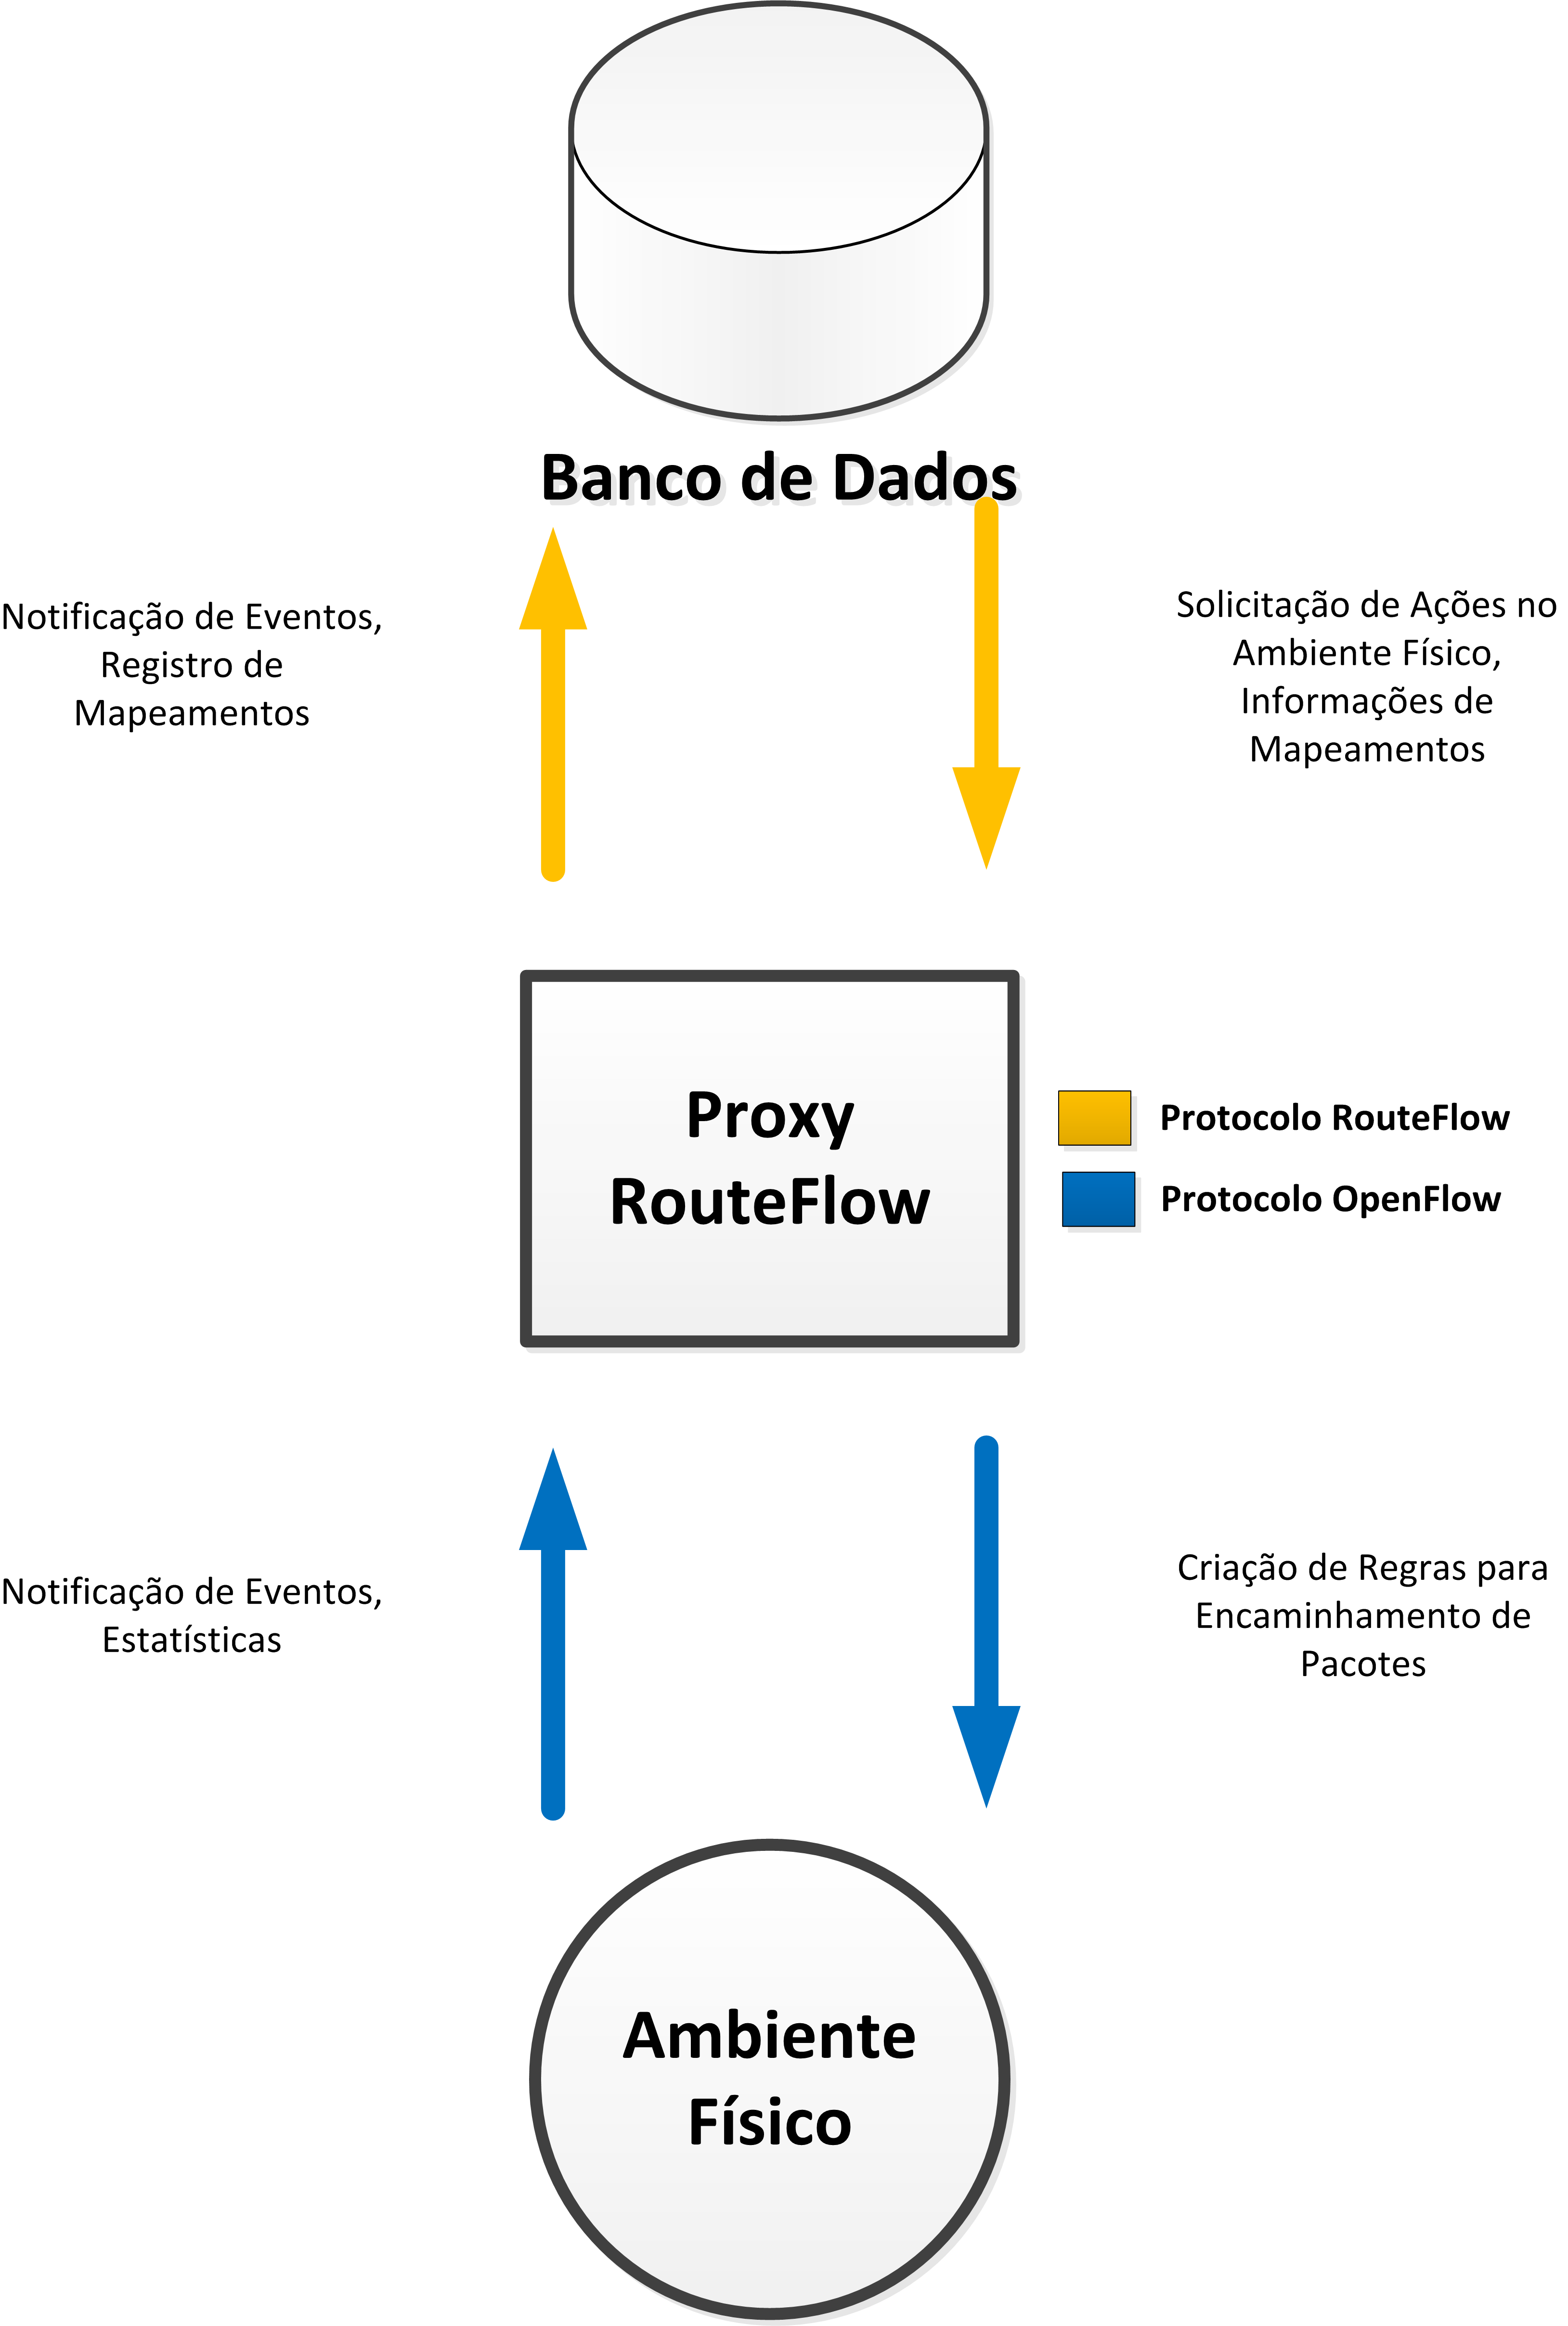
\includegraphics[width=120mm]{esquematico_geral_proxy.png}
\caption{Esquema Geral do Proxy RouteFlow (RFProxy).}
\label{fig:esquematicoProxy} 
\end{figure}
 

O próximo capitulo irá detalhas as funções internas e principais
estruturas do proxy RouteFlow.

\section{Descrição Geral da Estrutura do Proxy RouteFlow em Java}

Todos os componentes do proxy RouteFlow em Java foram agrupados em classes.
O agrupamento em classes facilitou a 
organização geral do código bem como a sua futura manutenção. 
Abaixo temos os principais componentes do proxy como 
suas respectivas descrições:

\begin{itemize}
\item \textit{MongoIPCMessageService:} Responsável pela
 comunicação entre o servidor RouteFlow e o proxy 
RouteFlow. A arquitetura básica do projeto RouteFlow 
faz uso de um banco de dados Não SQL para troca de 
mensagens entre seus componentes, sendo que o banco 
de dados escolhido foi o MongoDB. 

O MongoDB possui 
alto desempenho sendo totalmente escrito em C++, outro
 aspecto importante é o fato de não ser SQL, o 
que facilita a sua integração com as  principais linguagens
 de programação. 
O RouteFlow cria inúmeras tabelas no banco de dados, cada uma 
responsável pela comunicação entre um par 
de componentes, como toda comunicação é feita através de um 
sistema de banco de dados é possível que a 
comunicação entre componentes seja feita de forma simples, sem 
nenhum vinculo com a linguagem de 
implementação do mesmo. 

O componente MongoIPCMessageService 
cria um mecanismo de troca de mensagens entre processos (IPC) 
entre o servidor RouteFlow e o proxy RouteFlow. Os comandos são 
enviados de um componente para o outro 
na forma de mensagens pré-definidas. Cada mensagem define uma 
ação à ser tomada em relação aos eventos 
que vão ocorrendo ao longo da execução do ambiente físico e virtual. No corpo da 
mensagem estão os parâmetros que 
deverão ser usados para tomada da ação. Todas as mensagens que 
são colocadas na tabela pelo servidor RouteFlow 
possuem um campo que indica se a mesma já foi tratada e em caso 
negativo cabe ao proxy tomar a ação e 
atualizar o campo da mensagem. Para tratamento das mensagens é 
gerado uma thread em looping infinito 
cujo único proposito de existência é o tratamento de novas mensagens. 
Essa característica pretende ser melhorada nas próximas versões 
do RouteFlow;
\item \textit{RFProtocolFactory:} Responsável pela criação das 
mensagens do protocolo RouteFlow. Cada 
tipo de mensagem RouteFlow é representada por um código e 
por uma respectiva classe. É papel do 
RFProtocolFactory retornar os objetos de mensagens à partir de 
seu código. Esta estrutura facilita a 
inserção de novas mensagens no ambiente evitando a reprogramação 
de outras classes;
\item \textit{RFProtocolProcessor:} Responsável pelo processamento 
de mensagens vindas do servidor 
RouteFlow. Este componente define como será tratada cada mensagem 
vinda do servidor RouteFlow. As 
mensagens são lidas através do IPC e repassadas para tratamento.
\item \textit{AssociationTable:} Tabela mantida pelo proxy para armazenar 
a associação entre portas no 
ambiente virtual e portas no ambiente físico. A Tabela \ref{tab:tabela_associacao} nos 
mostra a estrutura básica da tabela de associação:

\begin{table}[h]
\centering
\begin{tabular}{|l|c|c|}
\hline
Tipo & Função\\
\hline
\hline
$dp_-id,\ dp_-port,\ vs_-id,\ vs_-port$ & Interface física com interface virtual\\
\hline
$vs_-id,\ vs_-port,\ dp_-id,\ dp_-port$ & Interface virtual com interface física\\
\hline
\end{tabular}
\caption{Representação da tabela de associação.}
\label{tab:tabela_associacao}
\end{table}

Repare que a Tabela \ref{tab:tabela_associacao} possui redundância
em suas colunas. Tal fato exige uma dupla atualização de campos
sempre que ocorre uma nova associação. Isso será resolvido
nas próximas versões do proxy.

\end{itemize} 

No Algoritmo abaixo temos uma visão geral da ideia usada para
construção do proxy, lembrando que a orientação a objetos
da linguagem Java força o código executável a ser construído
no formato de classe. Para deixar o código mais limpo, todas
as características especificas da linguagem Java foram omitidas,
deixando o código no formato de pseudo algoritmo.
\newline

%\begin{algorithmic}
\noindent
\tcc*[h]{Declaração dos componentes básicos.}
\newline

\noindent
\tcc*[h]{Provedor de serviços OpenFlow, fornecido pelo
controlador.}
\newline
\textit{floodlightProvider} $\leftarrow$ \textbf{IFloodlightProviderService};
\newline

\noindent
\tcc*[h]{Gerador de logs.}
\newline
\textit{logger} $\leftarrow$ \textbf{Logger};
\newline

\noindent
\tcc*[h]{Criação do mecanismo de comunicação
 entre processos, será explicado com mais detalhes.}
\newline
\textit{ipc} $\leftarrow$ \textbf{MongoIPCMessageService};
\newline

\noindent
\tcc*[h]{Gerador de mensagens RouteFlow. Cada mensagem RouteFlow
tem seu tipo e seus próprios parâmetros. Todas as mensagens
são representadas na forma de classes, a função em questão
basicamente retorna a classe representante da função de acordo
com o seu tipo.}
\newline
\textit{factory} $\leftarrow$ \textbf{RFProtocolFactory};
\newline

\noindent
\tcc*[h]{Processador de mensagens RouteFlow. Sera explicado
com mais detalhes.}
\newline
\textit{processor} $\leftarrow$ \textbf{RFProtocolProcessor};
\newline

\noindent
\tcc*[h]{Tabela de associação.}
\newline
\textit{table} $\leftarrow$ \textbf{AssociationTable};
\newline

\noindent
\tcc*[h]{Função usada para configurar regras, parcialmente fornecida
pelo controlador.}
\newline
\textit{\textbf{flowConfig()}};
\newline

\noindent
\tcc*[h]{Função usada para deletar regras, parcialmente fornecida
pelo controlador.}
\newline
\textit{\textbf{flowDelete()}};
\newline

\noindent
\tcc*[h]{Função usada para adicionar regras, parcialmente fornecida
pelo controlador.}
\newline
\textit{\textbf{flowAdd()}};
\newline

\noindent
\tcc*[h]{Função usada para registrar o proxy no
controlador Floodlight. Burocracia exigida pelo controlador.}
\newline
\textit{\textbf{init()}};
\newline

\noindent
\tcc*[h]{Função usada para o processamento dos pacotes
de entrada OpenFlow.}
\newline
\textit{\textbf{processPacketInMessage()}};
\newline

\noindent
\tcc*[h]{Função usada para iniciar a execução do proxy.
Burocracia exigida pelo controlador.}
\newline
\textit{\textbf{startUp()}};
\newline

\noindent
\tcc*[h]{Função usada para definir que tipo de mensagens 
OpenFlow serão tratadas pelo algoritmo do proxy e especificamente
por quais funções. O proxy habilita a função \textit{processPacketInMessage}
a tratar as mensagens de entrada OpenFlow.}
\newline
\textit{\textbf{receive()}};
\newline

\noindent
\tcc*[h]{Função executada sempre que um switch OpenFlow ingressa
na rede. Sempre que isso acontece é necessário informar
ao servidor RouteFlow as informações básicas do ingressante
para que o mesmo o associe a uma máquina virtual do
ambiente virtual.}
\newline
\textit{\textbf{addedSwitch()}};
\newline

\noindent
\tcc*[h]{Função executada sempre que um switch OpenFlow
abandona a rede. Sempre que isso acontece é necessário informar
ao servidor RouteFlow para o mesmo remova o registro e a
associação com a máquina virtual do ambiente virtual.}
\newline
\textit{\textbf{removedSwitch()}};
\newline

%\SetAlgoLined
%\Left$\leftarrow$ \FindCompress{$Im[i,j-1]$}\;
%\While{not at end of this document}{
%read current\;
%\eIf{understand}{
%go to next section\;
%current section becomes this one\;}
%{go back to the beginning of current section\;}
%}
%\caption{Ideia Básica do RFProxy}
%\label{alg:basico}
%\end{algorithmic}

Esse é o algoritmo básico do proxy RouteFlow. Todos os outros 
proxies implementados anteriormente seguem essa mesma
arquitetura.

Abaixo temos um pseudo algoritmo do mecanismo de comunicação
entre processos usado para funcionamento do proxy, no algoritmo
anterior a classe é chamada de \textbf{MongoIPCMessageService}:
\newline

\noindent
\tcc*[h]{Definição dos parâmetros de acesso ao
 banco de dados como nome da coleção de dados, nome
do banco de dados e endereço do banco de dados.}
\newline

\noindent
\tcc*[h]{Função usada para criação da thread não bloqueante
que executará a função ListenWorker. A função ListenWorker
será mostrada logo abaixo.}
\newline
\textit{\textbf{listen() \{}}
\newline
\tcc*[h]{Cria a nova thread, associa a função listenWorker e
inicia a sua execução.}
\newline
\textit{\textbf{\};}}
\newline

\noindent
\tcc*[h]{Função usada para checagem constante do banco
de dados à procura de alguma mensagem destinada
ao processo registrado. O processo se registra através da
criação de um canal de comunicação. O canal de comunicação
nada mais é que uma coleção de dados no banco de dados.}
\newline
\textit{\textbf{listenWorker() \{}}
\newline
\newline
\tcc*[h]{Define os parâmetros de busca. Os principais foram
definidos no início do algoritmo. É definido o nome da coleção
que será checada de tempos em tempos em busca de novas
mensagens.}
\newline
\newline
\indent
\textit{\textbf{enquanto(verdadeiro) \{}}
\newline
\indent
\indent
\textit{\textbf{se(mensagem não lida) \{}}
\newline
\indent
\indent
\indent
\tcc*[h]{Extrai os dados importantes e altera o parâmetro lido
do banco de dados para verdadeiro. Os dados são passados
para a função processor, mostrada no primeiro algoritmo.}
\newline
\indent
\indent
\textit{\textbf{\};}}
\newline
\indent
\indent
\textit{\textbf{senao \{}}
\newline
\indent
\indent
\indent
durma
\newline
\indent
\indent
\textit{\textbf{\};}}
\newline
\indent
\textit{\textbf{\};}}
\newline
\textit{\textbf{\};}}
\newline

\noindent
\tcc*[h]{Função usada para envio de dados ao banco de dados.
O termo envio significa inserir um novo conjunto de dados
na coleção. Serve basicamente para envio de mensagens à outros
processos.}
\newline
\textit{\textbf{send() \{}}
\newline
\textit{\textbf{\};}}
\newline

\noindent
\tcc*[h]{Função usada para criar um novo canal de comunicação.
Usada na primeira vez que o mecanismo de comunicação é
executado.}
\newline
\textit{\textbf{createChannel() \{}}
\newline
\textit{\textbf{\};}}
\newline

Este é basicamente a estrutura básica do algoritmo usado
para criação do mecanismo de comunicação entre processos.
A função listenWorker, sempre que nota o recebimento de
uma nova mensagem, encapsula os dados e transfere a função 
processor. A função processor, devido a orientação à objetos,
é sobrecarregada na definição do código do proxy. Assim é usada
para tomar as ações necessárias ao funcionamento do sistema.
Abaixo temos um pseudo código que será mais explicado a seguir:
\newline
\newline
\noindent
\tcc*[h]{Função usada para tratamento das mensagens
recebidas através do mecanismo de comunicação entre 
processos.}
\newline
\textit{\textbf{processor(dados) \{}}
\newline
\newline
\indent
\tcc*[h]{O parâmetro dados constitui basicamente do tipo
de mensagem e seus respectivos campos. Para cada tipo
de mensagem é necessário tomar uma ação.}
\newline
\indent
\textit{\textbf{caso(tipo) \{}}
\newline
\indent
\indent
tipo 1: \tcc*[h]{ação 1}
\newline
\indent
\indent
tipo 2: \tcc*[h]{ação 2}
\newline
\indent
\indent
...
\newline
\indent
\indent
tipo N: \tcc*[h]{ação N}
\newline
\indent
\textit{\textbf{\};}}
\newline
\textit{\textbf{\};}}
\newline

Esse é basicamente o algoritmo usado em todos os proxies RouteFlow.
As principais diferenças são relacionadas às linguagens de programação
 e ao controlador usado como interface com o protocolo
\textit{OpenFlow}.

\section{Descrição das Mensagens Traduzidas pelo Proxy RouteFlow}

Todas as mensagens mostradas na lista abaixo são representadas
via classes na linguagem Java. As classes foram geradas
automaticamente por um script em Python. Originalmente
o script só fazia a geração nas linguagens C++ e Python,
para que fossem utilizadas respectivamente pelos controladores
NOX e POX. Foi fruto desse trabalho de conclusão de curso
expandir o suporte do script para a linguagem Java. O script
é construído em Python e recebe como entrada uma lista com
a definição de campos e tipos de cada mensagem e retorna
os arquivos com as respectivas implementações. 

A Figura \ref{fig:mensagens}
ilustra o sentido de cada mensagem, nos dizendo que tipo de mensagem
é enviada para cada módulo. Vale lembra que as mensagens
são enviadas ao banco de dados centralizado para atuar no
mecanismo de troca de mensagens entre processos (IPC).
\newline

\begin{figure}[h] 
\centering
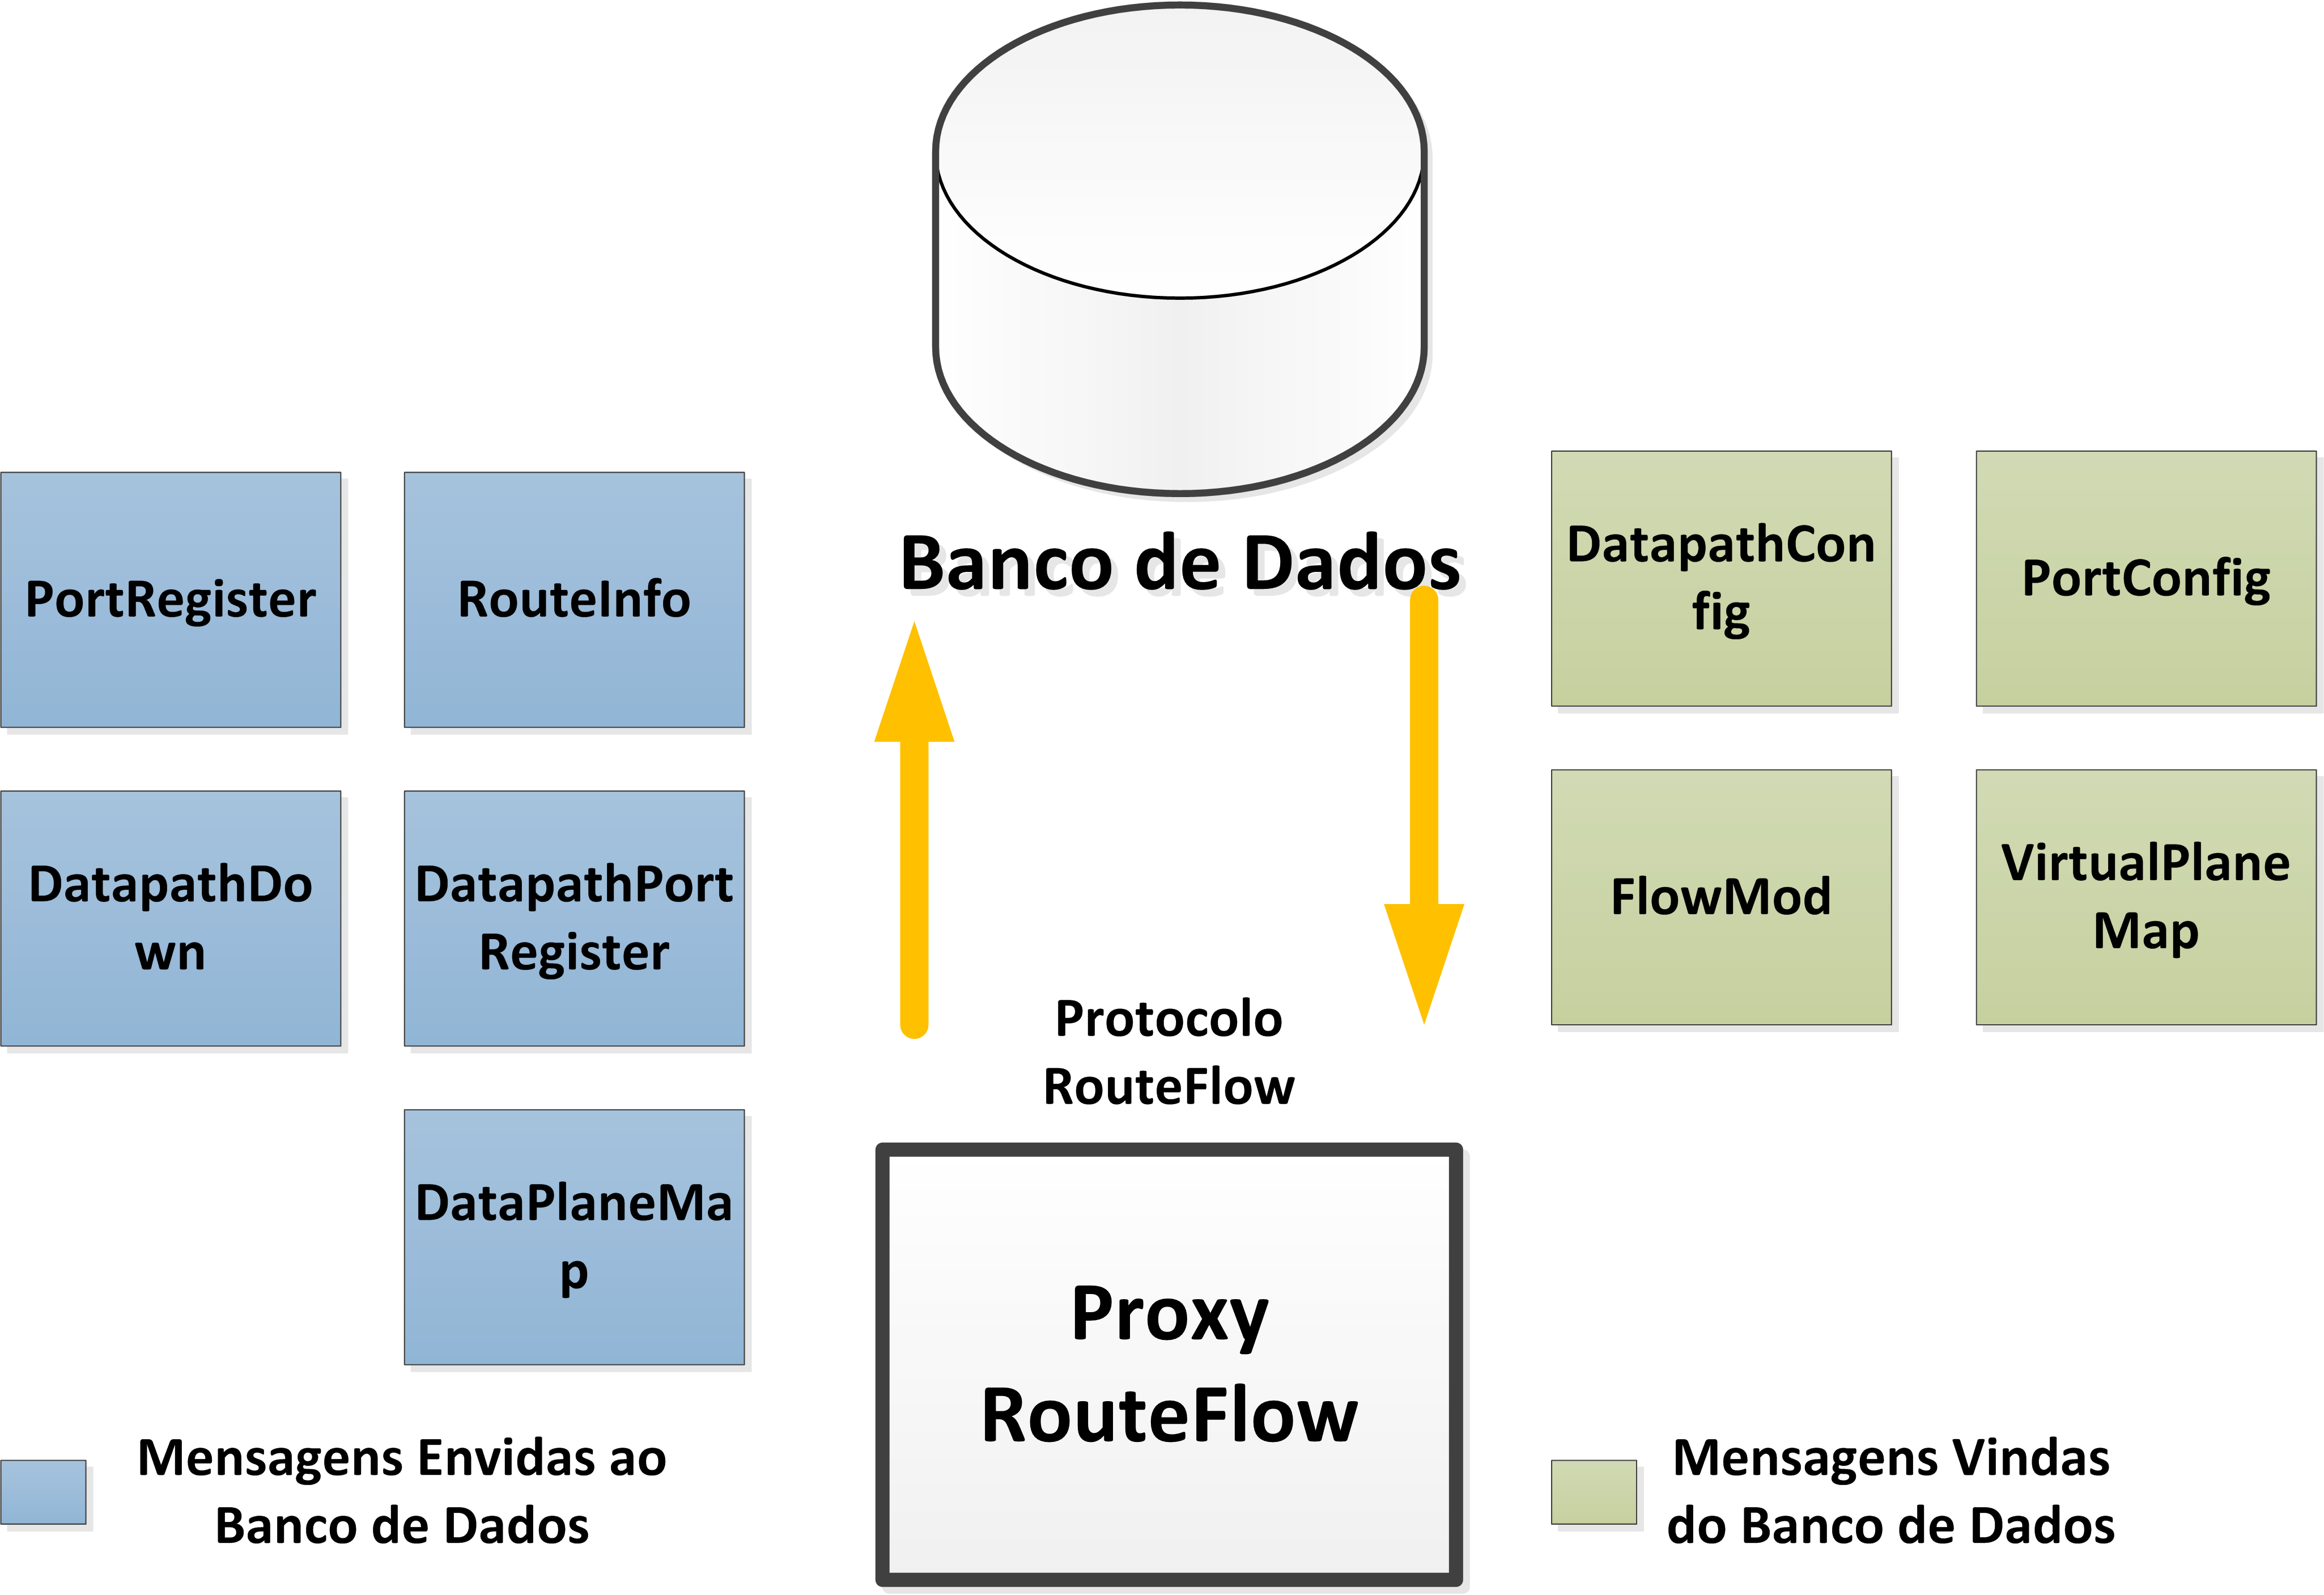
\includegraphics[width=140mm]{mensagens.png}
\caption{Fluxo das mensagens.}
\label{fig:mensagens} 
\end{figure}

\begin{itemize}
\item \textit{PortRegister:} mensagem utilizada sempre que um
novo \textit{switch} OpenFlow ingressa no ambiente físico. As mensagens 
servem para informar ao servidor RouteFlow sobre a disponibilidade
de portas para que as mesmas sejam associadas às interfaces
das máquinas virtuais no ambiente virtual.
\item \textit{PortConfig:} mensagem utilizada solicitação de 
configuração de alguma porta do ambiente físico pelo servidor
RouteFlow. Atualmente não é utilizada.
\item \textit{DatapathConfig:} mensagem utilizada para
configuração dos \textit{switches} via protocolo OpenFlow. A 
configuração envolve aspectos sobre como tratar certos tipos
de pacotes baseado em seus protocolos.
\item \textit{RouteInfo:} mensagem não utilizada.
\item \textit{FlowMod:} mensagem utilizada para 
solicitação da instalação de regras nos switches 
OpenFlow. As mensagens FlowMod possuem em seu 
corpo um conjunto de parâmetros que define uma nova regra 
a ser aplicada à um \textit{switch} OpenFlow. Cabe ao proxy 
criar a regra e envia-la corretamente ao \textit{switch}. 
Para envio das regras é necessário a manipulação do 
protocolo OpenFlow. O Floodlight fornece uma série de 
funções para esse proposito, sendo usado como uma 
API de comunicação entre os \textit{switches} OpenFlow e o 
proxy.
\item \textit{DatapathPortRegister:} mensagem utilizada 
para registrar as portas dos \textit{switches} OpenFlow 
no servidor RouteFlow. Esse registro é feito para que cada 
porta seja associada à uma porta da máquina 
virtual do ambiente virtual.
\item \textit{DatapathDown:} mensagem utilizada para que 
o proxy informe ao servidor RouteFlow sobre a 
desconexão de um \textit{switch} OpenFlow. O Floodlight, no papel 
de controlador OpenFlow, mantem um conjunto de 
informações à respeito dos \textit{switches} OpenFlow ativos, 
podendo detectar quedas nas conexões dos mesmos. O 
servidor RouteFlow necessita ter esse tipo de informação para 
possíveis alterações nas regras dos 
\textit{switches} OpenFlow.
\item \textit{VirtualPlaneMap:} mensagem utilizada para que 
o proxy associa cada porta do \textit{switch} 
OpenFlow à uma porta de uma máquina virtual no ambiente 
virtual.
\item \textit{DataPlaneMap:} mensagem utilizada para que o 
servidor RouteFlow informe ao proxy à 
respeito de uma associação de porta bem sucedida. O proxy 
mantém uma tabela de associação entre portas 
no ambiente virtual e portas no ambiente físico.
\end{itemize}


\chapter{Resultados}

\section{Resultados Preliminares}

Como principal resultado desse trabalho de conclusão de 
curso pode ser citado o suporte ao controlador Floodlight 
pelo Projeto RouteFlow. O Floodlight possui uma grande
comunidade de pesquisa e desenvolvimento sendo 
amplamente utilizado em redes de larga escala. Agora será
possível aos desenvolvedores do Floodlight executarem 
experimentos usando o ambiente provido pelo Projeto
RouteFlow.

Nas seções seguintes serão mostrados testes de desempenho
 e temporização de cada um dos proxies.

\section{Testes em Ambientes Virtuais}

Todos os testes dessa seção foram feitos em um ambiente 
virtual com as seguintes configurações: computador com
processador Intel Core i7 2630QM e 6GB de memória Ram 
DDR3, a ferramenta de virtualização escolhida foi o VMware
 Player executando uma máquina virtual com quatro núcleos 
e 1GB de memória Ram com o Ubuntu 11.04. Os testes 
mostrados abaixo foram executados para
todos os proxies do Projeto RouteFlow para que a 
virtualização tivesse o mesmo impacto sobre eles.

Para realização dos testes foi usado a ferramenta Cbench.
Um software especifico para testes de desempenho com 
controladores \textit{OpenFlow}. O programa basicamente
testa os controladores gerando eventos de entrada de 
pacotes para simulação de novos fluxos. O programa emula
 um conjunto de \textit{switches} que se conectam no 
controlador, enviam pacotes de entrada (\textit{packet-in})
e aguardam a instalação de novas regras (\textit{flow-mods}).

Os proxies são desenvolvidos usando os controladores como
interface de aplicação (API). Ao testarmos o desempenho 
de um controlador acoplado ao Projeto RouteFlow estaremos
testando na verdade o desempenho do proxy propriamente 
dito. As legendas das figuras e citações abaixo fazem
referência ao controlador que serviu de interface de programação
ao proxy, ou seja, ao mencionarmos os controladores NOX,
POX ou Floodlight estaremos na verdade mencionando
o proxy ao qual o controlador serviu de interface. 

A Figura \ref{fig:latencia1sw} mostra um teste com apenas
um \textit{switch} conectado. O ambiente montado pelo 
Projeto RouteFlow continha apenas uma máquina virtual
executando o software de roteamento Quagga. O teste em
questão leva em consideração uma distribuição cumulativa da
latência. Podemos notar que o desempenho do Floodlight é
parecido com o do NOX em uma grande parcela da distribuição.

\begin{figure}[h]
\centering
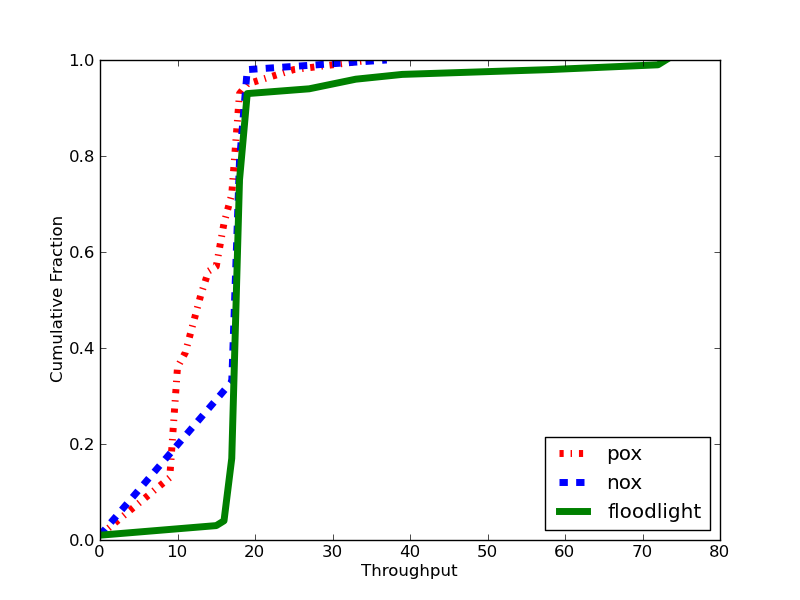
\includegraphics[width=140mm]{latencia_1sw.png}
\caption{Latência com um \textit{switch} em ms.}
\label{fig:latencia1sw} 
\end{figure}

A Figura \ref{fig:latencia4sw} foi obtida em um ambiente com
quatro \textit{switches} \textit{OpenFlow} conectados. O
ambiente RouteFlow tinha quatro máquinas virtuais executando
os algoritmos de roteamento, uma para cada \textit{switch OpenFlow},
isso pode ter afetado seriamente o desempenho mas para
o âmbito do trabalho de conclusão de curso estaremos 
testando apenas o desempenho de um proxy em relação ao
outro, sem levar em consideração o real desempenho de cada um
deles. Para termos dados reais de desempenho seria necessário
executar todos os procedimentos em um ambiente físico.
 Podemos ver
novamente que o desempenho do Floodlight é similar ao do
NOX em uma grande parcela da distribuição.

\begin{figure}[h]
\centering
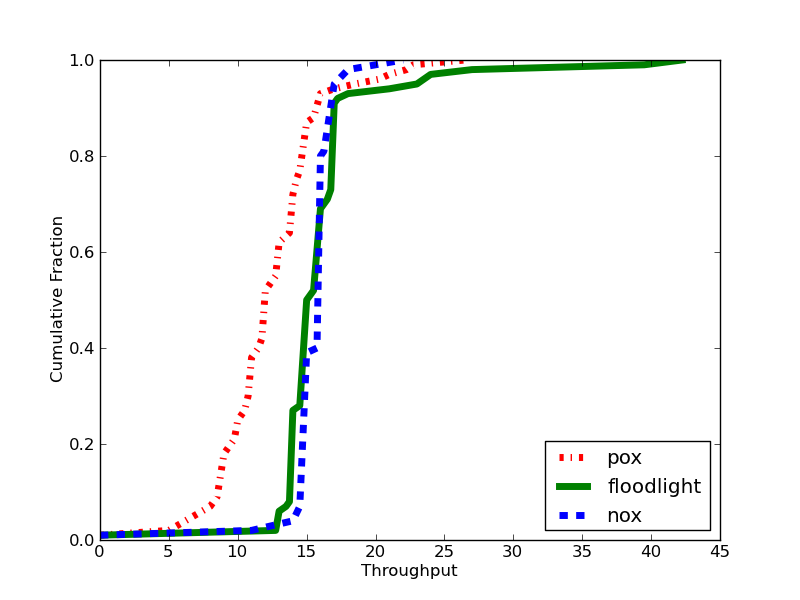
\includegraphics[width=140mm]{latencia_4sw.png}
\caption{Latência com quatro \textit{switches} em ms.}
\label{fig:latencia4sw} 
\end{figure}

Os próximos testes são uma distribuição cumulativa do
desempenho do controlador em termos criação de regras por
segundo. O ambiente é o mesmo dos testes anteriores.

A Figura \ref{fig:desempenho1sw} foi obtida em um ambiente
com apenas um \textit{switch OpenFlow}. Podemos observar 
que os três controladores tiveram desempenhos semelhantes.
Tal fato pode te ocorrido devido à dupla virtualização gerada
pela linguagem Java. Novas otimizações na forma de execução
da linguagem Java poderão contribuir para o aumento do 
desempenho do Floodlight.

\begin{figure}[h]
\centering
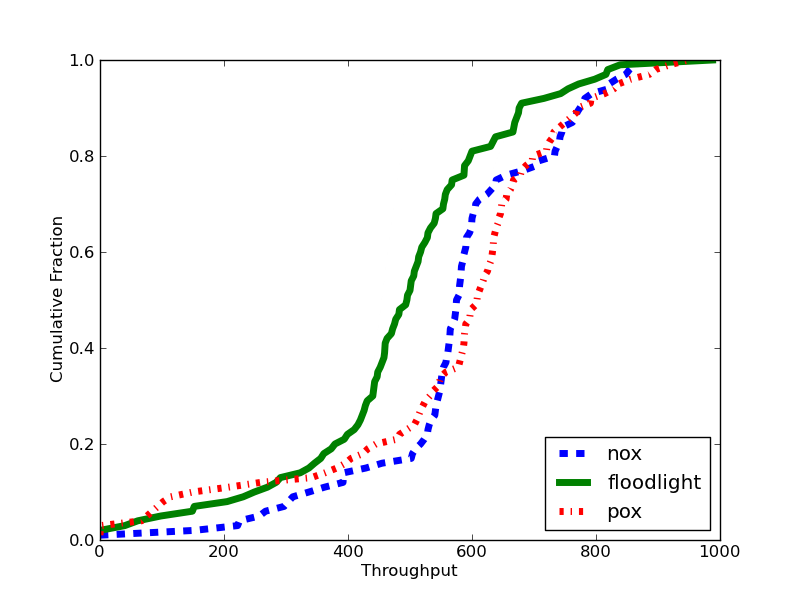
\includegraphics[width=140mm]{desempenho_1sw.png}
\caption{Desempenho com um \textit{switch} em fluxos por segundo.}
\label{fig:desempenho1sw} 
\end{figure}

A Figura \ref{fig:desempenho4sw} foi obtida em um ambiente
com quatro \textit{switches OpenFlow}. Novamente podemos
ver que o Floodlight teve desempenho parecido com o dos
outros proxies chegando a ser mais rápido que o NOX em 
alguns momentos.


\begin{figure}[h]
\centering
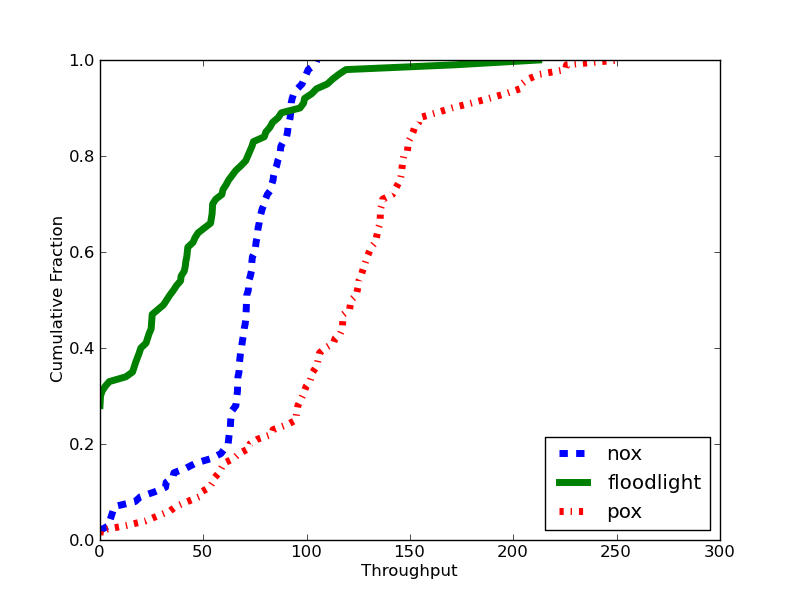
\includegraphics[width=140mm]{desempenho_4sw.png}
\caption{Desempenho com quatro \textit{switches} em fluxos por segundo.}
\label{fig:desempenho4sw} 
\end{figure}

Todos esses testes mostraram um desempenho similar entre
os três proxies levados em consideração, mostrando a viabilidade
de uso do proxy com Floodlight.

\section{Testes em Ambiente Reais}

Durante o desenvolvimento do trabalho de conclusão de
curso, um pesquisador do Departamento de Tecnologia de
Informação da Universidade Ghent (Bélgica) mostrou interesse
em usar o proxy RouteFlow com Floodlight para seus
experimentos. Parte dos experimentos foram feitos no ambiente
provido pelo Projeto OFELIA. Os experimentos
foram feitos com quatro \textit{switches OpenFlow}. Os testes
iniciais mostraram que o primeiro pacote levou cerca de 30ms
para chegar ao destino e os demais levaram cerca de
2ms, comprovando a instalação bem sucedida das regras pelo
proxy RouteFlow. O pesquisador não relatou nenhum 
problema ou inconsistência na rede, mostrando a operação
correta do proxy RouteFlow em Java.




\chapter{Conclusão}

\section{Trabalhos Futuros}

Como principal trabalho futuro estará a manutenção e 
inserção de novas funcionalidades no proxy RouteFlow.
Durante o desenvolvimento desse trabalho o Projeto
 RouteFlow ganhou suporte ao uso simultâneo de proxies, 
permitindo que cada trecho da rede seja controlado por um
proxy diferente. Tal funcionalidade exige a inserção de 
mais alguns parâmetros no código original desenvolvido
 durante o trabalho, sendo assim o próximo trabalho futuro.
A Figura \ref{fig:multiplosProxies} mostra de forma simples 
uma rede com tal funcionalidade habilitada:

\begin{figure}[h] 
\centering
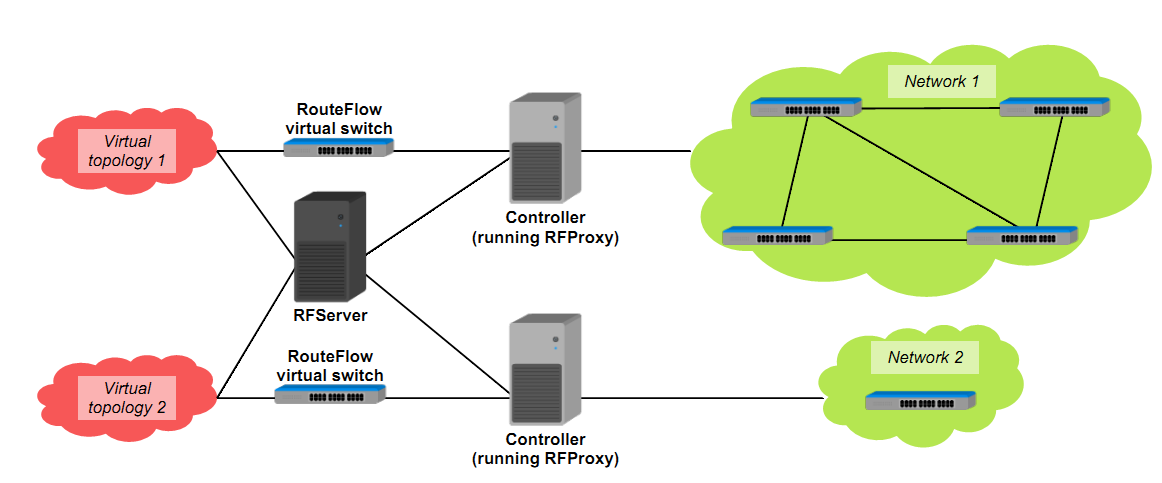
\includegraphics[width=160mm]{multiplosProxies.png}
\caption{Ambiente com inúmeros proxies e inúmeras redes.}
\label{fig:multiplosProxies} 
\end{figure}

Outro trabalho futuro será a remoção do looping infinito 
para leitura de mensagens vindas do servidor RouteFlow, 
um dos pesquisadores do Projeto RouteFlow está
desenvolvendo um mecanismo de comunicação mais ágil e
 eficaz. Esse mecanismo também deverá ser portado ao 
 novo proxy de forma a sempre se manter atualizado.

O site oficial do Projeto RouteFlow ainda descreve uma 
série de trabalhos que visam aumentar o desempenho do
sistema como um todo. Muitos exigirão a manutenção e 
atualização do proxy. Abaixo temos uma lista das principais
atualizações:

\begin{itemize}
\item \textit{Multiplexação de Roteadores:} mapeamento
de várias máquinas virtuais em um mesmo \textit{switch}
físico;
\item \textit{Aumento da Resiliência:} criação de um ambiente
de emergência que seria ativado em caso de falha do ambiente
principal;
\item \textit{Execução nas Nuvens:} execução do RouteFlow
em uma nuvens pública, como a disponibilizada pela Amazon.
\end{itemize}


\chapter{Agradecimentos}

\begin{itemize}
\item Allan Vidal -- CPqD, Campinas - SP
\item Cesar Augusto Cavalheiro Marcondes -- UFSCar, 
São Carlos - SP
\item Christian Esteve Rothenberg -- CPqD, Campinas - SP
\item Eder Leão Fernandes -- CPqD, Campinas - SP
\item Jorge Henrique de Barros Assumpção -- CPqD, Campinas - SP
\item Marcos Rogerio Salvador -- CPqD, Campinas - SP
\item Sachin Sharma -- Ghent, Bélgica
\item Toda a equipe do Forum do Floodlight
\end{itemize}

\bibliographystyle{abnt}
\nocite{*}
\bibliography{bare_conf}

\end{document}
